\chapter[NFSWEs 的任意高阶显式能量守恒方法]{NFSWEs 的任意高阶显式能量守恒方法
}

本文主要考虑具有周期性边界的非线性分数阶薛定谔波动方程的初边值问题

\begin{align}
&  u_{t t}+(-\Delta)^{\alpha / 2} u+\mathrm{i} \kappa u_{t}+\beta|u|^{2} u=0, \quad \boldsymbol{x} \in \Omega, \quad  t \in(0, T],\label{eq_SAVRRK:1}\\
& u(\boldsymbol{x}, 0)=u_{0}(\boldsymbol{x}), \quad u_{t}(\boldsymbol{x}, 0)=u_{1}(\boldsymbol{x}),\quad \boldsymbol{x} \in \Omega, \label{eq_SAVRRK:2}\\
& u(\boldsymbol{x}+\boldsymbol{L}, t)=u(\boldsymbol{x}, t), \quad t \in[0, T],\label{eq_SAVRRK:3}
\end{align}
其中,$\mathrm{i}=\sqrt{-1}$,$1<\alpha \leq 2$,$\kappa, \beta(>0)$为实常数,$u(\boldsymbol{x}, t)$是未知的复值函数,$u_{0}(\boldsymbol{x})$ 和 $u_{1}(\boldsymbol{x})$ 为已知的光滑函数,$\boldsymbol{x}\in\Omega\!\subset\!
R^d~(d\!=\!1,2)$,$\boldsymbol{L}$ 是周期.分数阶拉普拉斯算子可以通过傅里叶变换表示为
\begin{align}\label{eq_SAVRRK:4}
(-\Delta)^{\frac{\alpha}{2}} u(\boldsymbol{x},t)=\mathcal{F}^{-1}\left[|\boldsymbol{\xi}|^{\alpha} \mathcal{F}(u(\boldsymbol{\xi},t))\right],
\end{align}
其中,$\mathcal{F}$ 和 $\mathcal{F}^{-1}$ 分别表示傅里叶变换及其逆变换 \cite{caffarelliExtensionProblemRelated2007}.

设 $L^{p}(\Omega)$ 为定义在 $\Omega$ 上的可测复函数空间.定义内积和范数如下
\begin{equation}
(u, v)=\int_{\Omega} u \bar{v} \mathrm{~d} \boldsymbol{x}, \quad \|u\|_{L^{p}}=\left(\int_{\Omega}|u|^{p} d \boldsymbol{x}\right)^{\frac{1}{p}}, \quad 1 \leq p<\infty,
\label{eq_6}
\end{equation}
其中 $\bar{v}$ 表示 $v$ 的复共轭.

与许多其他基于物理场景的微分模型一样,所研究的具有周期性边界条件的NFSWEs \eqref{eq_SAVRRK:1}-\eqref{eq_SAVRRK:3}  具有如下两条守恒定律\cite{baoUniformErrorEstimates2012,ranLinearlyImplicitConservative2016}

质量守恒
\begin{align}\label{eq_PAVF:_8}
    G(t)=\kappa\|u(\cdot, t)\|^{2}+2\operatorname{Im}\left(u_{t}, u\right)=G(0), \quad t \in(0, T],
    \end{align}

能量守恒
\begin{align}\label{eq_SAVRRK:9}
	E(t)=\left\|u_{t}(\cdot, t)\right\|^{2}+\left\|(-\Delta)^{\frac{\alpha}{4}} u(\cdot, t)\right\|^{2}+\frac{\beta}{2}\|u(\cdot, t)\|_{L^{4}}^{4}=E(0), \quad t \in(0, T].
	\end{align}

\begin{proof}
	将方程 \eqref{eq_SAVRRK:1} 与 $u$做内积,并取虚部,有
\begin{equation}
\operatorname{Im}\left(u_{t t}, u\right)+\operatorname{Im}\left((-\Delta)^{\alpha / 2} u, u\right)+\operatorname{Im}\left(\mathrm{i} \kappa u_{t}, u\right)+\operatorname{Im}\left(\beta|u|^{2} u, u\right)=0 .
\label{eq_11}\end{equation}
不难验证
\begin{equation}
\operatorname{Im}\left(u_{t t}, u\right)=\frac{\mathrm{d}}{\mathrm{d} t} \operatorname{Im}\left(u_{t}, u\right), \operatorname{Im}\left(\mathrm{i} u_{t}, u\right)=\frac{1}{2} \frac{\mathrm{d}}{\mathrm{d} t}\|u(\cdot, t)\|_{L^{2}}^{2} .
\label{eq_12}\end{equation}
将方程 \eqref{eq_12} 代入方程 \eqref{eq_11} 得到
\begin{equation}
\kappa \frac{\mathrm{d}}{\mathrm{d} t}\|u(\cdot, t)\|_{L^{2}}^{2}+2 \frac{\mathrm{d}}{\mathrm{d} t} \operatorname{Im}\left(u_{t}, u\right)=0,
\label{eq_13}\end{equation}
此处使用了 $\operatorname{Im}\left((-\Delta)^{\alpha / 2} u, u\right)=0$,
详见 \cite{guoExistenceGlobalSmooth2008} 引理3.1的证明.

类似地,将方程 \eqref{eq_SAVRRK:1} 与 $u_{t}$ 做内积,并取实部,得到
\begin{equation}
\operatorname{Re}\left(u_{t t}, u_{t}\right)+\operatorname{Re}\left((-\Delta)^{\alpha / 2} u, u_{t}\right)+\operatorname{Re}\left(\mathrm{i} \kappa u_{t}, u_{t}\right)+\operatorname{Re}\left(\beta|u|^{2} u, u_{t}\right)=0 .
\label{eq_14}\end{equation}
其中$\operatorname{Im}(\cdot)$ 和 $\operatorname{Re}(\cdot)$ 分别表示复数的虚部和实部.容易验证
\begin{equation}
\operatorname{Re}\left(u_{t t}, u_{t}\right)=\frac{1}{2} \frac{\mathrm{d}}{\mathrm{d} t}\left\|u_{t}(\cdot, t)\right\|_{L^{2}}^{2}, \operatorname{Re}\left(|u|^{2} u, u_{t}\right)=\frac{1}{4} \frac{\mathrm{d}}{\mathrm{d} t}\|u(\cdot, t)\|_{L^{4}}^{4} .
\label{eq_15}\end{equation}
此外,有
\begin{equation}
\operatorname{Re}\left((-\Delta)^{\alpha / 2} u, u_{t}\right)=\frac{1}{2} \frac{\mathrm{d}}{\mathrm{d} t}\left\|(-\Delta)^{\alpha / 4} u(\cdot, t)\right\|_{L^{2}}^{2},
\label{eq_16}\end{equation}
参见 \cite{guoExistenceGlobalSmooth2008} 引理3.2的证明.
将方程 \eqref{eq_15} 和 \eqref{eq_16} 代入方程 \eqref{eq_14} 得到
\begin{equation}
\frac{\mathrm{d}}{\mathrm{d} t}\left\|u_{t}(\cdot, t)\right\|_{L^{2}}^{2}+\frac{\mathrm{d}}{\mathrm{d} t}\left\|(-\Delta)^{\alpha / 4} u(\cdot, t)\right\|_{L^{2}}^{2}+\frac{1}{2} \beta \frac{\mathrm{d}}{\mathrm{d} t}\|u(\cdot, t)\|_{L^{4}}^{4}=0 .
\label{eq_17}\end{equation}
其与方程 \eqref{eq_13} 分别意味着质量守恒 \eqref{eq_PAVF:_8}和能量守恒 \eqref{eq_SAVRRK:9}.

\end{proof}

\section{NFSWEs的SAV格式}\label{Section_SAVRRK: 2}

众所周知,所有的RK方法都可以保持任意线性不变量,只有辛RK方法能够保持任意二次不变量.
然而,并不存在标准RK方法可以保持高于二次的不变量或非多项式不变量.
为了克服这一限制并利用松弛RK方法保持二次不变量的特性,本节采用最近提出的SAV方法将NFSWEs \eqref{eq_SAVRRK:1}-\eqref{eq_SAVRRK:3} 以二次能量泛函的等价形式重新表述.

为了保证能量的正性,在 $\frac{\beta}{2}\|u(\cdot, t)\|_{L^{4}}^{4}$ 中添加一个正常数 $C_0$ 来修改式 \eqref{eq_SAVRRK:9} 中的能量.
鉴于$C_0$已知, 这种修改对于 \eqref{eq_SAVRRK:9} 中系统的能量不变性没有实质性影响.
因此,此处继续使用 $E(t)$ 表示修改后的能量,即
\begin{align}\label{eq_SAVRRK:9_1}
	E(t)\overset{\text{def}}{=}\left\|u_{t}(\cdot, t)\right\|^{2}+\left\|(-\Delta)^{\frac{\alpha}{4}} u(\cdot, t)\right\|^{2}+\frac{\beta}{2}\|u(\cdot, t)\|_{L^{4}}^{4} + C_0.
\end{align}
在此基础上,引入一个标量辅助变量
\begin{equation}
	w(t)\overset{\text{def}}{=}\sqrt{H(t)+C_0},
\end{equation}
这里$H(t)\overset{\text{def}}{=}\frac{\beta}{2}\|u(\cdot, t)\|_{L^{4}}^{4} .$
直接计算得到
\begin{align}
	w_t & =\frac{1}{2 \sqrt{H(t)+C_0}} \frac{d H(t)}{d t} \nonumber\\
	& =\frac{1}{2 \sqrt{H(t)+C_0}} \frac{d}{d t} \int_{\Omega} \frac{\beta}{2}|u|^{4}d \boldsymbol{x} \nonumber\\
	& =\frac{\beta}{\sqrt{H(t)+C_0}} \int_{\Omega} |u|^2 \operatorname{Re}\left(u \bar{u}_t\right) d \boldsymbol{x}\nonumber\\
	& =\operatorname{Re} \int_{\Omega} \frac{\beta|u|^2 u \bar{u}_t}{\sqrt{H(t)+C_0}} d \boldsymbol{x} \nonumber\\
	& =\operatorname{Re}\left(b(u), u_t\right), \label{eq_SAVRRK:2-1}
\end{align}
其中
\begin{align}
b(u)\overset{\text{def}}{=}\beta g(|u|^2) u / \sqrt{H(t)+C_0},
\end{align}


因此,NFSWEs \eqref{eq_SAVRRK:1}-\eqref{eq_SAVRRK:3} 可以等价地重新表述为
\begin{align}
& u_t=v, \label{eq_SAVRRK:2-2}\\
& v_t=-(-\Delta)^{\alpha / 2} u-\mathrm{i}\kappa v-b(u) w, \label{eq_SAVRRK:2-3}\\
& w_t=\operatorname{Re}\left(b(u), u_t\right),\label{eq_SAVRRK:2-4}
\end{align}
初始条件为
\begin{align}\label{eq_SAVRRK:31}
	u(\boldsymbol{x}, 0)=u_{0}(\boldsymbol{x}), \quad v(\boldsymbol{x}, 0)=u_{1}(\boldsymbol{x}), \quad w(0)=\sqrt{\frac{\beta}{2}\|u_{0}\|_{L^{4}}^{4} +C_0}.
\end{align}

将式 \eqref{eq_SAVRRK:2-2}和式\eqref{eq_SAVRRK:2-3} 分别与 $v_t$ , $u_t$ 做内积, 
式\eqref{eq_SAVRRK:2-4} 乘以 $w(t)$,然后对它们进行求和并在 $[0, t]$ 上积分,得到重构后的修正能量守恒定律
\begin{equation}
E(t)=\|v(\cdot, t)\|^2+\left\|(-\Delta)^{\frac{\alpha}{4}} u(\cdot, t)\right\|^{2}+w^2(t)=E(0),
\end{equation}
这与NFSWEs \eqref{eq_SAVRRK:1}-\eqref{eq_SAVRRK:3} 的原始能量守恒定律 \eqref{eq_SAVRRK:9} 本质上是一致的.

\section{傅里叶拟谱离散格式}\label{Section_SAVRRK: 3}
傅里叶拟谱法是解决偏微分方程的一种成熟技术, 它是非局部方法,
这与分数阶薛定谔方程中的分数阶拉普拉斯算子的非局部性质相契合.
傅里叶基函数是周期性边界条件下的拉普拉斯算子的特征函数,且快速傅里叶变换的使用使编程更加简便,可以大大减少计算量,提高计算效率.
因此,本文采用傅里叶拟谱法对等价系统 \eqref{eq_SAVRRK:2-2} - \eqref{eq_SAVRRK:31} 进行空间离散化.

不失一般性,设空间维度为2(即$d=2$). 对于正整数$M$和正偶数$N_{x}$、$N_{y}$,定义$\tau={T}/{M}$,$h_{x}={L}/{N_{x}}$,$h_{y}={L}/{N_{y}}$.令$\Omega_{h}=\left\{(x_{i}, y_{j}) \mid 0 \leq i \leq N_x-1;0 \leq j \leq N_y-1\right\}$,$\Omega_{\tau}=\left\{t_{m} \mid 0 \leq m \leq M\right\}$,$\Omega_{h}^{\tau}=\Omega_{h} \times \Omega_{\tau}$,
其中$x_{i}=i h_{x}$,$y_{j}=j h_{y}$,$t_{m}=m \tau$.
定义数值解在任意时间层$t_m$的向量形式为
\begin{align}\label{eq_SAVRRK:47}
&U^m=\left(u_{0,0}^m, \cdots, u_{N_{x}-1,0}^m, u_{0,1}^m, \cdots, u_{N_{x}-1,1}^m, \cdots, u_{0, N_{y}-1}^m, \cdots, u_{N_{x}-1, N_{y}-1}^m\right)^{T},\\
&V^m=\left(v_{0,0}^m, \cdots, v_{N_{x}-1,0}^m, v_{0,1}^m, \cdots, v_{N_{x}-1,1}^m, \cdots, v_{0, N_{y}-1}^m, \cdots, v_{N_{x}-1, N_{y}-1}^m\right)^{T},\\
&W^m=w^m.
\end{align}

对于定义在$\Omega_{h}$上的任意网格函数$u$和$v$,定义离散内积和相关的离散范数如下
\begin{align}\label{eq_SAVRRK:48}
(u, v)=h_{x} h_{y} \sum_{i=0}^{N_{x}-1} \sum_{j=0}^{N_{y}-1} u_{i, j} \bar{v}_{i, j},\quad\|u\|=(u, u)^{\frac{1}{2}},\quad\|u\|_{\infty}=\sup _{\left(x_{i}, y_{j}\right) \in \Omega_{h}}\left|u_{i, j}\right|.
\end{align}

设$\left(x_{i}, y_{j}\right)$为傅里叶插值点, $u_{N}(x, y)$为$u(x, y)$的插值多项式函数,其中
\begin{align}\label{eq_SAVRRK:50}
u_{N}(x, y)=\sum_{k_{1}=-N_{x} / 2}^{N_{x} / 2} \sum_{k_{2}=-N_{y} / 2}^{N_{y} / 2} \tilde{u}_{k_{1}, k_{2}} e^{\mathrm{i}\mu\left( k_{1} (x+L)+k_{2}(y+L)\right)},
\end{align}
这里$\mu={\pi}/{L}$, 系数
\begin{align}\label{eq_SAVRRK:51}
\tilde{u}_{k_{1}, k_{2}}=\frac{1}{N_{x} c_{k_{1}}} \frac{1}{N_{y} c_{k_{2}}} \sum_{l_1=0}^{N_{x}-1} \sum_{l_2=0}^{N_{y}-1} u(x_{l_1}, y_{l_2}) e^{-\mathrm{i}\mu\left( k_{1}(x_{l_1}+L)+k_{2}(y_{l_2}+L)\right)},
\end{align}
% 其中$c_{k_{1}}=1$对于$\left|k_{1}\right|<N_{x}/2$,$c_{k_{2}}=1$对于$\left|k_{2}\right|<N_{y}/2$,$c_{k_{1}}=2$对于$k_{1}=\pm N_{x}/2$,$c_{k_{2}}=2$对于$k_{2}=\pm N_{y}/2$.
其中
\begin{align}c_{k_1} = \begin{cases} 1, & \text{if } |k_1| < \frac{N_x}{2} \\ 2, & \text{if } |k_1| = \frac{N_x}{2} \end{cases} \quad , \quad c_{k_2} = \begin{cases} 1, & \text{if } |k_2| < \frac{N_y}{2} \\ 2, & \text{if } |k_2| = \frac{N_y}{2} \end{cases}.\end{align}
因此
% 分数阶拉普拉斯算子 $-(-\Delta)^{\frac{\alpha}{2}} u(x, y)$ 可以通过以下逼近得到:
\begin{align}\label{eq_SAVRRK:52}
-(-\Delta)^{\frac{\alpha}{2}} u_{N}\left(x, y\right)=-\sum\limits_{k_{1}=-N_{x} / 2}^{N_{x} / 2} \sum\limits_{k_{2}=-N_{y} / 2}^{N_{y} / 2}\left|\left(k_{1} \mu\right)^{2}+\left(k_{2} \mu\right)^{2}\right|^{\frac{\alpha}{2}} \tilde{u}_{k_{1}, k_{2}} e^{\mathrm{i}\mu\left( k_{1} (x+L)+k_{2}(y+L)\right)}.
\end{align}
将式\eqref{eq_SAVRRK:51} 插入 式\eqref{eq_SAVRRK:52},并考虑在点$(x_i,y_j)$处得到的方程
\begin{align}
&-(-\Delta)^{\frac{\alpha}{2}} u_{N}\left(x_{i}, y_{j}\right)\nonumber\\
=&\sum\limits_{l_{1}=0}^{N_{x}-1} \sum\limits_{l_{2}=0}^{N_{y}-1}u(x_{l_{1}}, y_{l_{2}})\Big(-\sum\limits_{k_{1}=-N_{x} / 2}^{N_{x} / 2} \sum\limits_{k_{2}=-N_{y} / 2}^{N_{y} / 2} \frac{1}{N_{x} c_{k_{1}}} \frac{1}{N_{y} c_{k_{2}}}\left|\mu^{2} \cdot \mathbf{k}^{2}\right|^{\frac{\alpha}{2}} e^{\mathrm{i} \mu\left(k_{1}\left(x_{i}-x_{l_{1}}\right)+k_{2}\left(y_{j}-y_{l_{2}}\right)\right)}\Big)\nonumber\\
=&\left(D^{\alpha}U\right)_{i+j N_{x}},\label{eq_SAVRRK:53}
\end{align}
其中$\mu^{2} \cdot \mathbf{k}^{2}=\mu^{2}\left(k_{1}^{2}+k_{2}^{2}\right)$,$D^{\alpha}$ 是具有以下元素的谱对称微分矩阵
\begin{align}\label{eq_SAVRRK:54}
\left(D^{\alpha}\right)_{i+j N_{x}, l_{1}+l_{2} N_{x}}=-\sum\limits_{k_{1}=-N_{x} / 2}^{N_{x} / 2} \sum\limits_{k_{2}=-N_{y} / 2}^{N_{y} / 2}\frac{1}{N_{x} c_{k_{1}}} \frac{1}{N_{y} c_{k_{2}}}\left|\mu^{2} \cdot \mathbf{k}^{2}\right|^{\frac{\alpha}{2}} e^{\mathrm{i}\mu\left(k_{1}\left(x_{i}-x_{l_{1}}\right)+k_{2}\left(y_{j}-y_{l_{2}}\right)\right)}.
\end{align}

将傅里叶拟谱法应用于之前的等价系统 \eqref{eq_SAVRRK:2-2} - \eqref{eq_SAVRRK:2-4},得到如下空间半离散系统
\begin{align}
 U_t&=V, \label{eq_SAVRRK:3-9}\\
 V_t&=D^{\alpha} U-\mathrm{i}\kappa V- b(U) \cdot W, \label{eq_SAVRRK:3-10}\\
 W_t&=\operatorname{Re}\left(b(U), U_t\right),\label{eq_SAVRRK:3-11}
\end{align}
其初始条件为$U^0, V^0, W^0$,这里的$\cdot$表示向量之间的点乘.

对于空间半离散系统 \eqref{eq_SAVRRK:3-9} - \eqref{eq_SAVRRK:3-11},有以下定理.

\begin{theorem}	\label{thm3}
空间半离散系统 \eqref{eq_SAVRRK:3-9}-\eqref{eq_SAVRRK:3-11} 具有半离散二次能量守恒律
\begin{equation}
\frac{dE}{dt}=0, \label{eq_SAVRRK:313a}
\end{equation}
其中
\begin{equation}
E(U,V,W)\overset{\text{def}}{=}\|V\|^2 + \|D^\frac{\alpha}{2} U\|^2+\left(W\right)^2.\label{eq_SAVRRK:313}
\end{equation}
\end{theorem}

\begin{proof}
	将式 \eqref{eq_SAVRRK:3-9} 和 式\eqref{eq_SAVRRK:3-10} 分别与 $V_t$ 和 $U_t$ 做内积, 
	同时将式 \eqref{eq_SAVRRK:3-11} 乘以 $W$,得到以下方程:
\begin{align}
\left(V_t, U_t\right)&=\left(V_t, V\right), \label{eq_SAVRRK:313a}\\
\left(V_t, U_t\right)&=\left(D^{\alpha} U, U_t\right)-\mathrm{i} \kappa\left(V, U_t\right)-W\left(b(U), U_t\right), \label{eq_SAVRRK:313b}\\
W W_t&=W\operatorname{Re}\left(b(U), U_t\right).\label{eq_SAVRRK:313c}
\end{align}
将方程 \eqref{eq_SAVRRK:313a}-\eqref{eq_SAVRRK:313c} 相加,得到
\begin{equation}
\left(V_t, V\right) + W W_t= \left(D^{\alpha} U, U_t\right)-\mathrm{i} \kappa\left(V, U_t\right)-W\left(b(U), U_t\right) + W\operatorname{Re}\left(b(U), U_t\right).
\end{equation}
取实部得
% \begin{align}
% \operatorname{Re}\left(V_t, V\right) + \operatorname{Re}\left(W W_t\right)&= \operatorname{Re}\left(D^{\alpha} U, U_t\right)-\operatorname{Re}\left(\mathrm{i} \kappa\left(V, U_t\right)\right)-W\operatorname{Re}\left(b(U), U_t\right) + W\operatorname{Re}\left(b(U). U_t\right).
% \end{align}
% 因此,
\begin{align}
\operatorname{Re}\left(V_t, V\right) + \operatorname{Re}\left(W W_t\right)&= \operatorname{Re}\left(D^{\alpha} U, U_t\right).\label{eq_SAVRRK:319}
\end{align}
注意到
\begin{equation}
\operatorname{Re}\left(V_t, V\right) = \frac{1}{2}\frac{d }{d t}\|V\|^2, \quad \operatorname{Re}\left(W W_t\right) = \frac{1}{2}\frac{d }{d t}\left(W\right)^2,\quad \operatorname{Re}\left(D^{\alpha} U, U_t\right)=-\frac{1}{2}\frac{d }{d t}\|D^\frac{\alpha}{2}U\|^2,\label{eq_SAVRRK:320}
\end{equation}
将 \eqref{eq_SAVRRK:320} 代入 \eqref{eq_SAVRRK:319} 得到
\begin{equation}
\frac{d }{d t}\left(\|V\|^2+\|D^\frac{\alpha}{2}U\|^2+\left(W\right)^2\right)=0.
\end{equation}
证毕.
\end{proof}

\section{显式 SAV-RRK 方法}\label{Section_SAVRRK: 4}
% 本节旨在介绍基于SAV方法的NFSWEs的不变量守恒显式RRK方法.
% 首先回顾RRK方法并讨论它们的保结构性质.

% \subsection{显式SAV-RRK方案}
为简洁起见,引入以下符号
\begin{equation}
	\begin{aligned}
		\bm{y}&=\left(U,V,W\right)^T,\quad\bm{y}_0=\left(U^0,V^0,W^0\right)^T , \\
		\bm{f}&=(f^1,f^2,f^3)^T\overset{\text{def}}{=}(V,D^{\alpha} U-\mathrm{i}\kappa V-b(U)\cdot W,\operatorname{Re}\left(b(U), U_t\right))^T.
	\end{aligned}
\end{equation}
于是,基于SAV方法的半离散系统\eqref{eq_SAVRRK:3-9}-\eqref{eq_SAVRRK:3-11}可以重写为
\begin{equation}
\left\{\begin{array}{l}
\bm{y}_t=\bm{f}(\bm{y}),\quad t \in(0, T],\\
\bm{y}(0)=\bm{y}_0.
\end{array}\right.\label{eq_SAVRRK:3-121}
\end{equation}
设$\bm{y}^m$是$\bm{y}\left(t_m\right)$的近似.系统\eqref{eq_SAVRRK:3-121}的$s$级显式RK格式\cite{hairerRungeKuttaMethods2015}为
\begin{equation}
\left\{\begin{array}{l}
\bm{Y}_{m i}=\bm{y}^m+\tau \sum\limits_{j=1}^{i-1} a_{i j} \bm{f}_{m j}, \quad i=1, \ldots, s, \\
\bm{y}^{m+1}=\bm{y}^m+\tau \sum\limits_{i=1}^s b_i \bm{f}_{m i},
\end{array}\right.\label{eq_SAVRRK:4-31}
\end{equation}
其中$\bm{f}_{m j}=\bm{f}\left(\bm{Y}_{m j}\right)$,$j=1, \ldots, s$.
定义矩阵$A$和向量$b$如下
\begin{equation}
\begin{aligned}
A & =\left(a_{i j}\right)_{s \times s}, \quad a_{i j}=0 \quad \text {对于} \quad j \geq i, \\
b & =\left(b_1, \cdots, b_s\right)^T.
\end{aligned}
\end{equation}
于是$s$级显式SAV-RK格式可以用Butcher表表示为
\begin{equation}
\begin{array}{c|c}
c & A \\
\hline \\
& b^T
\end{array},
\end{equation}
其中向量$c=(c_1,c_2,\dots,c_s)$满足$c_i=\sum\limits_{j=1}^s a_{i j}$,$i=1, \ldots, s$.

然而,众所周知,只有特定的隐式RK方法才可能是辛的或代数上稳定的,不存在辛的或代数稳定的显式RK方法.
这导致任何标准显式SAV-RK方法无法保持原始问题\eqref{eq_SAVRRK:3-121}的能量守恒特性.
因此,引入松弛RK技术.具体而言,考虑在区间$\left[\hat{t}_m, \hat{t}_{m+1}\right], m \geq 0$上的单步操作,设$\bm{y}_\gamma^m=\left(U^{m}_{\gamma},V^{m}_{\gamma},W^{m}_{\gamma}\right)^T$是$\bm{y}\left(\hat{t}_m\right)$的数值逼近,
对于系统\eqref{eq_SAVRRK:3-121},$s$级显式SAV-RRK方法定义为
\begin{equation}
\left\{\begin{array}{l}
\bm{Y}_{m i}=\bm{y}_\gamma^m+\tau \sum\limits_{j=1}^{i-1} a_{i j} \bm{f}_{m j}, \quad i=1, \ldots, s, \\
\bm{y}_\gamma^{m+1}=\bm{y}_\gamma^m+\gamma_m \tau \sum\limits_{i=1}^s b_i \bm{f}_{m i}.
\end{array}\right.\label{eq_SAVRRK:4-3}
\end{equation}
同样,$s$级RRK方法\eqref{eq_SAVRRK:4-3}可以用Butcher表表示为
\begin{equation}
\begin{array}{c|c}
c & A \\
\hline \\
& \tilde{b}^T
\end{array},
\end{equation}
其中$\tilde{b}=\gamma_m b$,$\gamma_m\neq 0$, 并且满足:
\begin{equation}
\left\{\begin{array}{ll}
E_{\gamma}^{m+1}=E_{\gamma}^{m}, & \text{若} \quad  \sum\limits_{i=1}^s b_i \bm{f}_{m i} \neq 0,\\
\gamma_m=1, & \text{若} \quad  \sum\limits_{i=1}^s b_i \bm{f}_{m i} =0,
\end{array}\right.\label{eq_SAVRRK:4-6}
\end{equation}
这里
\begin{align}\label{eq_SAVRRK:4-6b}
E_{\gamma}^{m}  =\|V_{\gamma}^{m}\|^2+\|D^\frac{\alpha}{2} U_{\gamma}^{m}\|^2+\big(W_{\gamma}^{m}\big)^2.
\end{align}

显式SAV-RRK方法\eqref{eq_SAVRRK:4-3}的一个显著优势在于可以通过调整参数$\gamma_m$ 使其达到能量守恒的目的.
实际上,从式\eqref{eq_SAVRRK:4-6}中可知,当$\sum\limits_{i=1}^s b_i \bm{f}_{m i}=0$时,取$\gamma_m=1$.当$\sum\limits_{i=1}^s b_i \bm{f}_{m i}\neq 0$时,
\begin{align}
E_{\gamma}^{m+1}  = & \|V_{\gamma}^{m}\|^2+\|D^\frac{\alpha}{2} U_{\gamma}^{m}\|^2+\big(W_{\gamma}^{m}\big)^2 \nonumber\\
& + \big(V_{\gamma}^{m},\gamma_m\tau\sum\limits_{i=1}^{s}b_if_{mi}^2\big)+\big(\gamma_m\tau\sum\limits_{i=1}^{s}b_if_{mi}^2,V_{\gamma}^{m}\big)\nonumber\\
&-\big(U_{\gamma}^{m}, D^{\alpha}\big(\gamma_m\tau\sum\limits_{i=1}^{s}b_if_{mi}^1\big)\big)-\big(\gamma_m\tau\sum\limits_{i=1}^{s}b_if_{mi}^1, D^{\alpha} U_{\gamma}^{m}\big)\nonumber\\
&+2W_{\gamma}^{m}\gamma_m\tau\sum\limits_{i=1}^{s}b_if_{mi}^3+\big(\gamma_m\tau\sum\limits_{i=1}^{s}b_if_{mi}^3\big)^2.\label{eq_SAVRRK:49}
\end{align}
将其与\eqref{eq_SAVRRK:4-6}结合,得到
\begin{align*}
&\gamma_m\tau\big[\big(V_{\gamma}^{m},\sum\limits_{i=1}^{s}b_if_{mi}^2\big)+\big(\sum\limits_{i=1}^{s}b_if_{mi}^2,V_{\gamma}^{m}\big)-\big(U_{\gamma}^{m},D^{\alpha}\big(\sum\limits_{i=1}^{s}b_if_{mi}^1\big)\big)-\big(\sum\limits_{i=1}^{s}b_if_{mi}^1, D^{\alpha} U_{\gamma}^{m}\big)\\
&+2W_{\gamma}^{m}\sum\limits_{i=1}^{s}b_if_{mi}^3\big] +\gamma_m^2\tau^2\big[\big\|\sum\limits_{i=1}^{s}b_if_{mi}^2\big\|^2+ \big\|D^\frac{\alpha}{2}\big(\sum\limits_{i=1}^{s}b_if_{mi}^1\big)\big\|^2+\big(\sum\limits_{i=1}^{s}b_if_{mi}^3\big)^2\big]=0,
\end{align*}
这是关于$\gamma_m$的二次方程.注意到$\gamma_m\neq 0$,因此可得
\begin{equation}\label{eq_SAVRRK:r1}\small
\gamma_m \!=\! \frac{\big(\!V_{\gamma}^{m},\sum\limits_{i=1}^{s}b_if_{mi}^2\!\big)\!+\!\big(\!\sum\limits_{i=1}^{s}b_if_{mi}^2,V_{\gamma}^{m}\!\big)\!-\!\big(\!U_{\gamma}^{m},D^{\alpha}\big(\sum\limits_{i=1}^{s}b_if_{mi}^1\big)\!\big)\!-\!\big(\!\sum\limits_{i=1}^{s}b_if_{mi}^1, D^{\alpha} U_{\gamma}^{m}\!\big)\!+\!2W_{\gamma}^{m}\sum\limits_{i=1}^{s}b_if_{mi}^3}{-\tau\big[\big\|\sum\limits_{i=1}^{s}b_if_{mi}^2\big\|^2+\big\|D^\frac{\alpha}{2}\big(\sum\limits_{i=1}^{s}b_if_{mi}^1\big)\big\|^2+\big(\sum\limits_{i=1}^{s}b_if_{mi}^3\big)^2\big]} .
\end{equation}
这意味着当$\sum\limits_{i=1}^s b_i \bm{f}_{m i}\neq 0$时,$\gamma_m$的值也可以通过式\eqref{eq_SAVRRK:r1}显式计算确定.

实际上,定义在\eqref{eq_SAVRRK:4-6}中的$\gamma_m$的值在$\tau\rightarrow 0$时接近于$1$,这将在\ref{Section_SAVRRK: 5-1}节中进一步讨论.
因此,显式SAV-RRK方法\eqref{eq_SAVRRK:4-3}是良定的.此外,很容易证明该方法具有以下定理中描述的能量守恒律.
\begin{theorem}
设显式SAV-RK方法\eqref{eq_SAVRRK:4-31}的阶数至少为2,则显式SAV-RRK方法\eqref{eq_SAVRRK:4-3}的解满足
\begin{equation}
E_{\gamma}^{m+1}=E_{\gamma}^{m}, \label{eq_SAVRRK:4-10}
\end{equation}
其中$E_{\gamma}^{m}$由式\eqref{eq_SAVRRK:4-6b}定义.
\end{theorem}

\begin{proof}
当$\sum\limits_{i=1}^s b_i \bm{f}_{m i}=0$时,根据\eqref{eq_SAVRRK:4-3}中的第二个方程可知, $\bm{y}_\gamma^{m+1}\equiv\bm{y}_\gamma^m$,它自动满足式\eqref{eq_SAVRRK:4-10}.
对于$\sum\limits_{i=1}^s b_i \bm{f}_{m i}\neq 0$的情况,可从条件\eqref{eq_SAVRRK:4-6}中得到式\eqref{eq_SAVRRK:4-10}.证毕.
\end{proof}

\section{显式SAV-RRK方法的精度}\label{Section_SAVRRK: 5}
在本节中,将讨论显式SAV-RRK方法\eqref{eq_SAVRRK:4-3}的精度.为此,首先估计松弛因子$\gamma_m$,它在接下来的分析中起着关键作用.
虽然松弛因子$\gamma_m$往往在不同时间层会发生变化,但可通过类似的方式在不同步骤上进行估计.
因此,这里只考虑作区间$\left[\hat{t}_m, \hat{t}_{m+1}\right]$内的讨论.

\subsection{松弛因子的估计}\label{Section_SAVRRK: 5-1}

因为$\sum\limits_{i=1}^s b_i \bm{f}_{m i} = 0$的情况很简单, 本文将仅关注$\sum\limits_{i=1}^s b_i \bm{f}_{m i} \neq 0$的情况.
令
\begin{equation}
\begin{aligned}\label{eq_SAVRRK:sm}
S_m(\gamma)=&\big\|V_\gamma^m+\gamma \tau \sum\limits_{i=1}^s b_i \bm{f}_{m i}^2\big\|^2 + \big\|D^\frac{\alpha}{2} \big(U_\gamma^m+\gamma \tau \sum\limits_{i=1}^s b_i \bm{f}_{m i}^1\big)\big\|^2\\
&+\big(W_\gamma^m+\gamma \tau \sum\limits_{i=1}^s b_i \bm{f}_{m i}^3\big)^2-\|V_\gamma^{m}\|^2 - \|D^\frac{\alpha}{2} U_\gamma^{m}\|^2-\big(W_\gamma^{m}\big)^2,
\end{aligned}
\end{equation}
则式\eqref{eq_SAVRRK:4-6}中定义的$\gamma_m$的值恰好是函数$S_m(\gamma)$的非零根.
此外,关于$S_m(\gamma)$有以下结果.
\begin{lemma}\label{lem_SAVRRK:5_1}
设显式SAV-RK方法\eqref{eq_SAVRRK:4-31}的阶数为$p$,则有
\begin{equation}
S_m(1)=\mathcal{O}(\tau^{p+1}).
\end{equation}
\end{lemma}

\begin{proof}
类似于\cite{liImplicitexplicitRelaxationRungeKutta2022}中引理3.1的证明,
考虑初值问题
\begin{equation}
\left\{\begin{array}{l}
\tilde{\bm{y}}^{\prime}=\bm{f}(\tilde{\bm{y}}), \quad t \geq \hat{t}_m, \\
\tilde{\bm{y}}\left(\hat{t}_m\right)=\bm{y}_\gamma^m,
\end{array}\right.
\end{equation}
其中$\bm{y}_\gamma^m$是显式SAV-RRK方法\eqref{eq_SAVRRK:4-3}的解.
通过使用显式SAV-RRK方法\eqref{eq_SAVRRK:4-3}进行单步计算,得到数值解$\bm{y}_\gamma^{m+1}$.根据式\eqref{eq_SAVRRK:sm},有
\begin{equation}
\begin{aligned}
S_m(\gamma) \!=& \|V_\gamma^{m+1}\|^2 \!+\! \|D^\frac{\alpha}{2} U_\gamma^{m+1}\|^2\!+\!\big(W_\gamma^{m+1}\big)^2\!-\!\|V_\gamma^{m}\|^2 \!-\! \|D^\frac{\alpha}{2} U_\gamma^{m}\|^2\!-\!\big(W_\gamma^{m}\big)^2\\
\!=& \|V_\gamma^{m+1}\|^2 \!+\! \|D^\frac{\alpha}{2} U_\gamma^{m+1}\|^2\!+\!\big(W_\gamma^{m+1}\big)^2\!-\!\|\tilde{V}(\hat{t}_{m})\|^2 \!-\! \|D^\frac{\alpha}{2} \tilde{U}(\hat{t}_{m})\|^2\!-\!\big(\tilde{W}(\hat{t}_{m})\big)^2.
\end{aligned}
\end{equation}

从$\bm{y}_\gamma^m$开始,对于充分小的$\tau$, 显式SAV-RK方法\eqref{eq_SAVRRK:4-31}生成具有$p$阶精度的数值解$\tilde{\bm{y}}^{m+1}$,
即$\tilde{\bm{y}}^{m+1}=\tilde{\bm{y}}\left(\hat{t}_m+\tau\right)+\mathcal{O}\left(\tau^{p+1}\right)$.
值得注意的是,当$\gamma=1$时,由式\eqref{eq_SAVRRK:4-3}定义的显式SAV-RRK方法将简化为由式\eqref{eq_SAVRRK:4-31}描述的显式SAV-RK方法.也就是说,$\bm{y}_\gamma^{m +1}=\tilde{\bm{y}}^{m +1}$.因此,可以得到
\begin{align}
S_m(1) = &\|\tilde{V}^{m+1}\|^2 + \|D^\frac{\alpha}{2} \tilde{U}^{m+1}\|^2+\big(\tilde{W}^{m+1}\big)^2-\|\tilde{V}(\hat{t}_{m})\|^2 - \|D^\frac{\alpha}{2} \tilde{U}(\hat{t}_{m})\|^2-\big(\tilde{W}(\hat{t}_{m})\big)^2 \nonumber\\
= &\|\tilde{V}^{m+1}\|^2 -\|\tilde{V}(\hat{t}_{m}+\tau)\|^2 +\|\tilde{V}(\hat{t}_{m}+\tau)\|^2-\|\tilde{V}(\hat{t}_{m})\|^2\nonumber\\
& + \|D^\frac{\alpha}{2} \tilde{U}^{m+1}\|^2 -\|D^\frac{\alpha}{2} \tilde{U}(\hat{t}_{m}+\tau)\|^2+\|D^\frac{\alpha}{2} \tilde{U}(\hat{t}_{m}+\tau)\|^2- \|D^\frac{\alpha}{2} \tilde{U}(\hat{t}_{m})\|^2\nonumber\\
& +\big(\tilde{W}^{m+1}\big)^2 -\big(\tilde{W}(\hat{t}_{m}+\tau)\big)^2+\big(\tilde{W}(\hat{t}_{m}+\tau)\big)^2-\big(\tilde{W}(\hat{t}_{m})\big)^2 \nonumber\\
= &\mathcal{O}\big(\tau^{p+1}\big) +2\int_{\hat{t}_m}^{\hat{t}_m+\tau}\big[\operatorname{Re}\big(V_t, V\big) + \operatorname{Re}\big(W W_t\big) - \operatorname{Re}\big(D^{\alpha} U, U_t\big)\big]dt.\label{eq_SAVRRK:54}
\end{align}
将式\eqref{eq_SAVRRK:319}代入方程\eqref{eq_SAVRRK:54}即可完成证明.
\end{proof}

根据引理 \ref{lem_SAVRRK:5_1},可以得到以下关于松弛因子 $\gamma_m$ 的估计.

\begin{theorem}\label{thm_SAVRRK:5_1}
设显式 SAV-RK 方法 \eqref{eq_SAVRRK:4-31} 的阶数为 $p~(p \geq 2)$,那么式 \eqref{eq_SAVRRK:4-6} 中定义的松弛因子 $\gamma_m$ 满足
\begin{equation}\label{eq_SAVRRK:5_3}
\gamma_m=1+\mathcal{O}(\tau^{p-1}).
\end{equation}
\end{theorem}	

\begin{proof}
根据 $\sum\limits_{i=1}^s b_i \bm{f}_{m i}$ 的值分别考虑两种情况.

情况 1:当 $\sum\limits_{i=1}^s b_i \bm{f}_{m i} = 0$ 时,根据式 \eqref{eq_SAVRRK:4-6} 中 $\gamma_m$ 的定义,有 $\gamma_m = 1$,这显然满足 \eqref{eq_SAVRRK:5_3}.

情况 2:当 $\sum\limits_{i=1}^s b_i \bm{f}_{m i} \neq 0$ 时,由式 \eqref{eq_SAVRRK:49} 可得
\begin{align}\label{eq_SAVRRK:5_4a}
	S_m(\gamma)=&~E_{\gamma}^{m+1}-E_{\gamma}^{m}\nonumber\\
	=&~\gamma\tau\Big[(V_{\gamma}^{m},\sum\limits_{i=1}^{s}b_if_{mi}^2)+(\sum\limits_{i=1}^{s}b_if_{mi}^2,V_{\gamma}^{m})-(U_{\gamma}^{m},D^{\alpha} (\sum\limits_{i=1}^{s}b_if_{mi}^1))-(\sum\limits_{i=1}^{s}b_if_{mi}^1, D^{\alpha} U_{\gamma}^{m})\nonumber\\
	&+2W_{\gamma}^{m}\sum\limits_{i=1}^{s}b_if_{mi}^3\Big]+\gamma^2\tau^2\Big[\|\sum\limits_{i=1}^{s}b_if_{mi}^2\|^2+ \|D^\frac{\alpha}{2}(\sum\limits_{i=1}^{s}b_if_{mi}^1)\|^2+(\sum\limits_{i=1}^{s}b_if_{mi}^3)^2\Big].
\end{align}
注意到 $S_m(\gamma)$ 是 $\gamma$ 的二次函数,它有非零根
\begin{equation}\label{eq_SAVRRK:5_4a3}\small
	\gamma=\!\frac{\tau\Big[(V_{\gamma}^{m},\sum\limits_{i=1}^{s}b_if_{mi}^2)\!+\!(\sum\limits_{i=1}^{s}b_if_{mi}^2,V_{\gamma}^{m})\!-\!(U_{\gamma}^{m},D^{\alpha} (\sum\limits_{i=1}^{s}b_if_{mi}^1))\!-\!(\sum\limits_{i=1}^{s}b_if_{mi}^1, D^{\alpha} U_{\gamma}^{m})\!+\!2W_{\gamma}^{m}\sum\limits_{i=1}^{s}b_if_{mi}^3\Big]}{-\tau^2\Big[\|\sum\limits_{i=1}^{s}b_if_{mi}^2\|^2\!+\! \|D^\frac{\alpha}{2}(\sum\limits_{i=1}^{s}b_if_{mi}^1)\|^2\!+\!(\sum\limits_{i=1}^{s}b_if_{mi}^3)^2\Big]}.
\end{equation}
根据引理 \ref{lem_SAVRRK:5_1},有
\begin{align}\label{eq_SAVRRK:5_4a2}
	S_m(1)=&\tau\Big[(V_{\gamma}^{m},\sum\limits_{i=1}^{s}b_if_{mi}^2)+(\sum\limits_{i=1}^{s}b_if_{mi}^2,V_{\gamma}^{m})-(U_{\gamma}^{m},D^{\alpha} (\sum\limits_{i=1}^{s}b_if_{mi}^1))-(\sum\limits_{i=1}^{s}b_if_{mi}^1, D^{\alpha} U_{\gamma}^{m})\nonumber\\
	&+2W_{\gamma}^{m}\sum\limits_{i=1}^{s}b_if_{mi}^3\Big]+\tau^2\Big[\|\sum\limits_{i=1}^{s}b_if_{mi}^2\|^2+ \|D^\frac{\alpha}{2}(\sum\limits_{i=1}^{s}b_if_{mi}^1)\|^2+(\sum\limits_{i=1}^{s}b_if_{mi}^3)^2\Big],
\end{align}
其阶数为$\mathcal{O}(\tau^{p+1})$ .
定义 $\tilde{\bm{f}}_m=\bm{f}\left(\bm{y}\left(\tilde{t}_m\right)\right)$,那么当 $\tau\rightarrow 0$ 时,有 $\bm{f}_{m i}=\tilde{\bm{f}}_m+\mathcal{O}(\tau)$.
因此,有
\begin{align}\label{eq_SAVRRK:5_4a4}
	&\tau^2\Big[\|\sum\limits_{i=1}^{s}b_if_{mi}^2\|^2+ \|D^\frac{\alpha}{2}(\sum\limits_{i=1}^{s}b_if_{mi}^1)\|^2+(\sum\limits_{i=1}^{s}b_if_{mi}^3)^2\Big]\nonumber\\
	=&\tau^2\Big[\|\sum\limits_{i=1}^{s}b_i\tilde{f}_{mi}^2\|^2+ \|D^\frac{\alpha}{2}(\sum\limits_{i=1}^{s}b_i\tilde{f}_{mi}^1)\|^2+(\sum\limits_{i=1}^{s}b_i\tilde{f}_{mi}^3)^2\Big]+\mathcal{O}(\tau^3)\nonumber\\
	=&\mathcal{O}(\tau^2).
\end{align}
将 \eqref{eq_SAVRRK:5_4a4} 和 \eqref{eq_SAVRRK:5_4a2} 代入 \eqref{eq_SAVRRK:5_4a3} 中,得到
\begin{align}\label{eq_SAVRRK:5_4a5}
	\gamma&=1+\frac{\mathcal{O}(\tau^{p+1})}{-\tau^2\Big[\|\sum\limits_{i=1}^{s}b_if_{mi}^2\|^2+ \|D^\frac{\alpha}{2}(\sum\limits_{i=1}^{s}b_if_{mi}^1)\|^2+(\sum\limits_{i=1}^{s}b_if_{mi}^3)^2\Big]}\nonumber\\
	&=1+\frac{\mathcal{O}(\tau^{p+1})}{\mathcal{O}(\tau^2)}\nonumber\\
	&=1+\mathcal{O}(\tau^{p-1}).
\end{align}
证毕.
\end{proof}

\begin{remark}\label{rk_SAVRRK:5_1}
定理 \ref{thm_SAVRRK:5_1} 表明,当 $\tau\rightarrow 0$ 时,松弛因子 $\gamma_m$ 接近于 $1$,
这意味着松弛RK方法可以被视为标准RK方法的小扰动.
\end{remark}

\subsection{显式SAV-RRK方法的截断误差}
基于定理\ref{thm_SAVRRK:5_1}给出的松弛因子$\gamma_m$的估计, 本小节进一步研究显式SAV-RRK方法\eqref{eq_SAVRRK:4-3}的精度.

在这之前,将显式SAV-RRK方法\eqref{eq_SAVRRK:4-3}重新表示为
\begin{equation}
\left\{\begin{array}{l}
\bm{Y}_{m i}=\bm{y}_\gamma^m+\tau \sum\limits_{j=1}^{i-1} a_{i j} \bm{f}_{m j}, \quad i=1, \ldots, s, \\
\bm{y}^{m+1}=\bm{y}_\gamma^m+\tau \sum\limits_{i=1}^s b_i \bm{f}_{m i},\\
\bm{y}_\gamma^{m+1}=\bm{y}^{m+1}+\left(\gamma_m-1\right)\left(\bm{y}^{m+1}-\bm{y}_\gamma^m\right) .
\end{array}\right.\label{eq_SAVRRK:4-321}
\end{equation}
前两个方程本质上构成标准的显式SAV-RK方法.

数值解$\bm{y}_\gamma^{m+1}$在$\hat{t}_{m+1}$处可以从如下两种角度进行解释\cite{ketchesonRelaxationRungeKutta2019}%即增量方向技术(IDT)和松弛技术(RT).
\begin{itemize}
\item 增量方向技术(IDT)的角度:$\bm{y}_\gamma^{m+1}$被视为对$\bm{y}\left(\hat{t}_m+\tau\right)$的近似,当$m \geq 0$,$\hat{t}_m=t_m$.
\item 松弛技术(RT)的角度:$\bm{y}_\gamma^{m+1}$被视为对$\bm{y}\left(\hat{t}_m+\gamma_m \tau\right)$的近似,当$m>0$时,$\hat{t}_m$可能不等于$t_m$.
\end{itemize}

值得注意的是, 对数值解$\bm{y}_\gamma^{m+1}$的不同解释可能导致不同的收敛结果.
参考\cite{ranochaGeneralRelaxationMethods2020}中引理2.7的证明思路,得到了以下结果.

\begin{theorem}\label{thm_SAVRRK:5_4}
设显式SAV-RK方法\eqref{eq_SAVRRK:4-31}的阶数为$p~(p \geq 2)$, 则有
\begin{itemize}
\item 对于IDT,显式SAV-RRK方法\eqref{eq_SAVRRK:4-3}的阶数为$p-1$.
\item 对于RT,显式SAV-RRK方法\eqref{eq_SAVRRK:4-3}的阶数为$p$.
\end{itemize}
\end{theorem}


\begin{proof}
设$\hat{t}_{m i}=\hat{t}_m+c_i\tau, i=1, \ldots, s$,
则从式\eqref{eq_SAVRRK:4-321}中的第二个方程可以得到
\begin{equation}\label{eq_SAVRRK:4-321b}
\bm{y}\left(\hat{t}_m+\tau\right)=\bm{y}\left(\hat{t}_m\right)+\tau \sum_{i=1}^s b_i \bm{f}\left(\bm{y}\left(\hat{t}_{m i}\right)\right)+\mathcal{O}\left(\tau^{p+1}\right).
\end{equation}
%\textcolor[rgb]{0.00,0.07,1.00}{这是从显式SAV-RK方法\eqref{eq_SAVRRK:4-31}的精度推导出来的.}

为了估计式\eqref{eq_SAVRRK:4-321}中第三个方程的截断误差.
定义
$$\phi_m(\bm{y}(t))\overset{\text{def}}{=}\bm{y}\left(\hat{t}_m\right)+\tau \sum\limits_{i=1}^s b_i \bm{f}\left(\bm{y}\left(\hat{t}_{m i}\right)\right),$$
以及
\begin{equation}
\bm{y}\left(\hat{t}_{m+1}\right)=\phi_m(\bm{y}(t))+\left(\gamma_m-1\right)\left(\phi_m(\bm{y}(t))-\bm{y}\left(\hat{t}_m\right)\right)+T_{m+1}.
\end{equation}
利用定理\ref{thm_SAVRRK:5_1}中给出的$\gamma_m=1+\mathcal{O}\left(\tau^{p-1}\right)$,可以从\eqref{eq_SAVRRK:4-321b}中得到
%one can obtain that
\begin{equation}
\begin{aligned}
T_{m+1}= & \bm{y}\left(\hat{t}_{m+1}\right)\!-\!\phi_m(\bm{y}(t))\!-\!\left(\gamma_m-1\right)\left(\phi_m(\bm{y}(t))\!-\!\bm{y}\left(\hat{t}_m\right)\right) \\
= & \bm{y}\left(\hat{t}_{m+1}\right)\!-\!\left(\bm{y}\left(\hat{t}_m\!+\!\tau\right)\!-\!\mathcal{O}(\tau^{p+1})\right)\!-\!\left(\gamma_m-1\right)\left(\bm{y}\left(\hat{t}_m+\tau\right)\!-\!\mathcal{O}(\tau^{p+1})\!-\!\bm{y}\left(\hat{t}_m\right)\right) \\
= & \bm{y}\left(\hat{t}_{m+1}\right)\!-\!\bm{y}\left(\hat{t}_m\!+\!\tau\right)\!-\!\left(\gamma_m-1\right)\left(\bm{y}\left(\hat{t}_m+\tau\right)\!-\!\bm{y}\left(\hat{t}_m\right)\right)\!+\!\mathcal{O}(\tau^{p+1})\!+\!\mathcal{O}((\gamma_m-1) \tau^{p+1}) \\
= & \bm{y}\left(\hat{t}_{m+1}\right)\!-\!\bm{y}\left(\hat{t}_m\!+\!\tau\right)\!-\!\left(\gamma_m-1\right) \bm{y}^{\prime}\left(\hat{t}_m+\tau\right) \tau\!+\!\mathcal{O}((\gamma_m-1) \tau^2)\!+\!\mathcal{O}(\tau^{p+1}) \\
= & \bm{y}\left(\hat{t}_{m+1}\right)\!-\!\bm{y}\left(\hat{t}_m\!+\!\tau\right)\!-\!\left(\gamma_m-1\right) \bm{y}^{\prime}\left(\hat{t}_m+\tau\right) \tau\!+\!\mathcal{O}(\tau^{p+1}).
\end{aligned}
\end{equation}

对于IDT,$\bm{y}_\gamma^{m+1}$被视为在$\hat{t}_m+\tau$处的近似,因此$\hat{t}_{m+1}=\hat{t}_m+\tau$,这意味着
$$T_{m+1}=-\left(\gamma_m-1\right) \bm{y}^{\prime}\left(\hat{t}_m+\tau\right) \tau+\mathcal{O}\left(\tau^{p+1}\right)=\mathcal{O}\left(\tau^p\right).$$
也就是说,方法\eqref{eq_SAVRRK:4-3}的阶数为$p-1$阶(IDT角度).

对于RT,由于$\bm{y}_\gamma^{m+1}$被视为在$\hat{t}_m+\gamma_m \tau$处的近似.再次使用上述估计中的Taylor展开,有
\begin{align}
T_{m+1}\!= & \bm{y}\left(\hat{t}_m\!+\!\tau\!+\!\left(\gamma_m\!-\!1\right) \tau\right)\!-\!\bm{y}\left(\hat{t}_m\!+\!\tau\right)\!-\!\left(\gamma_m\!-\!1\right) y^{\prime}\left(\hat{t}_m\!+\!\tau\right) \tau\!+\!\mathcal{O}(\tau^{p+1}) \nonumber\\
\!= & \bm{y}\left(\hat{t}_m\!+\!\tau\right)\!+\!\left(\gamma_m\!-\!1\right) \bm{y}^{\prime}\left(\hat{t}_m\!+\!\tau\right) \tau\!+\!\mathcal{O}(\left(\gamma_m\!-\!1\right)^2 \tau^2)\!\nonumber\\
&-\!\bm{y}\left(\hat{t}_m\!+\!\tau\right)\!-\!\left(\gamma_m\!-\!1\right) \bm{y}^{\prime}\left(\hat{t}_m\!+\!\tau\right) \tau\!+\!\mathcal{O}(\tau^{p+1}) \nonumber\\
\!= & \mathcal{O}(\tau^{p+1}).
\end{align}
这意味着方法\eqref{eq_SAVRRK:4-3}的阶数为$p$阶(RT角度).
\end{proof}

\begin{remark}\label{rk_SAVRRK:5_5}
在实际计算过程中,IDT角度的阶数可能高于预期,甚至可以达到RT角度的阶数,这可以在算例\ref{exp_SAVRRK:1}中观察到.
\end{remark}
	
\begin{remark}\label{rk_SAVRRK:5_6}
本章提出的方法很容易拓展到其他类似的分数阶方程,例如非线性分数阶波动方程和分数阶Klein-Gordon-Schr{\"o}dinger方程等,详见算例\ref{exp_SAVRRK:3}-\ref{exp_SAVRRK:4}.
\end{remark}

\section{数值算例}\label{Section_SAVRRK: 6}

本节中将通过数值算例展示显式SAV-RRK方法\eqref{eq_SAVRRK:4-3}的精度和守恒性质.

不失一般性的,在计算中使用了以下的显式RK方法\cite{shuEfficientImplementationEssentially1988}
\begin{itemize}
\item $\operatorname{RK}(2,2)$:二级二阶Heun方法%\cite{shuEfficientImplementationEssentially1988}.
\begin{equation}
\begin{array}{c|cc}
0 & 0 & 0 \\
\frac{2}{3} & \frac{2}{3} & 0 \\
\hline & \frac{1}{4} & \frac{3}{4}
\end{array}.
\end{equation}
	
\item $\mathrm{RK}(3,3)$:三级三阶Heun方法%\cite{shuEfficientImplementationEssentially1988}.
	
\begin{equation}
\begin{array}{c|ccc}
0 & 0 & 0 & 0 \\
\frac{1}{3} & \frac{1}{3} & 0 & 0 \\
\frac{2}{3} & 0 & \frac{2}{3} & 0 \\
\hline & \frac{1}{4} & 0 & \frac{3}{4}
\end{array}.
\end{equation}
		
\item $\operatorname{RK}(4,4)$:四级四阶Gill方法%\cite{shuEfficientImplementationEssentially1988}.
		
\begin{equation}
\begin{array}{c|cccc}
0 & 0 & 0 & 0 & 0 \\
\frac{1}{2} & \frac{1}{2} & 0 & 0 & 0 \\
\frac{1}{2} & \frac{\sqrt{2}-1}{2} & 1-\frac{\sqrt{2}}{2} & 0 & 0 \\
1 & 0 & -\frac{\sqrt{2}}{2} & 1+\frac{\sqrt{2}}{2} & 0 \\
\hline & \frac{1}{6} & \frac{2-\sqrt{2}}{6} & \frac{2+\sqrt{2}}{6} & \frac{1}{6}
\end{array}.
\end{equation}
\end{itemize}

值得一提的是,本章的主要关注点是时间方向精度.因此,这里没有展示空间方向精度.
另外,鉴于数值算例中能量的固有正性,在计算中简单地设置常数$C_0=0$.

时间方向上的误差和收敛阶通过以下方式计算
\begin{equation}
	\text{Error}(\tau) = \|U_{N}^{M} - U_{N}^{2 M}\|_{\infty},~\text{order} = \log_{2}\left[\frac{\text{Error}(\tau)}{\text{Error}(\tau / 2)}\right].\label{eq_SAVRRK:104}
\end{equation}

为了展示守恒性能,定义相对能量误差:
\begin{equation}\label{eq_SAVRRK:105}
	R E_{\gamma}^{m} = \left|\frac{E_{\gamma}^{m} - E_{\gamma}^{0}}{E_{\gamma}^{0}}\right|,
\end{equation}
其中$E_{\gamma}^{m}$表示时刻$t_m$处的离散能量.

\begin{example}\label{exp_SAVRRK:1} 
	考虑一维NFSWEs \eqref{eq_SAVRRK:1}-\eqref{eq_SAVRRK:3},形式如下\cite{ranLinearlyImplicitConservative2016}
	\begin{equation}\label{eq_SAVRRK:108}
		u_{t t}+(-\Delta)^{\alpha / 2} u+\mathrm{i}u_t+|u|^2 u=0, \quad (x,t)\in  (-25, 25)\times[0, T],
	\end{equation}
	其中 $u(x, 0)=(1+\mathrm{i}) x e^{-10(1-x)^2}$ 且 $u_t(x, 0)=0$.
	\end{example}
	不失一般性,取 $\alpha=1.5$ 、 $T=1$. %,以确认显式SAV-RRK方法\eqref{eq_SAVRRK:4-3}的精度.
	表 \ref{tab_SAVRRK:6-1} 展示了标准SAV-RK、SAV-RRK(RT)和SAV-RRK(IDT)方法在时间方向上的误差和收敛阶.
	可以看到,所有的SAV-RRK(RT)方法在收敛阶与标准SAV-RK方法保持一致,而SAV-RRK(IDT)方法表现不同.
	SAV-RRK(IDT)(2,2) 和 SAV-RRK(IDT)(4,4) 展示出了比在定理\ref{thm_SAVRRK:5_4}中预期阶数更高的收敛阶.
	而 SAV-RRK(IDT)(3,3) 并没有出现升阶现象.这种不同的行为可能归因于 $\max\limits _m\left|\gamma_m-1\right|$ 
	的收敛阶对于 SAV-RRK(RT)(2, 2) 和 SAV-RRK(RT)(4, 4) 提高了一个阶,如图 \ref{fig_SAVRRK:1} 所示.


\begin{table}[H]\scriptsize
\centering
\caption{当 $N=32$,$T = 1$ 时,算例 \ref{exp_SAVRRK:1} 在时间方向的误差和收敛阶}
\begin{tabular}{lllllrlrlrlrlrl}
\toprule
\multicolumn{2}{l}{\multirow{2}[3]{*}{\textbf{RK(Stage,Order)}}} & \multicolumn{2}{l}{\multirow{2}[3]{*}{$\bm{\tau}$}} & \multicolumn{3}{c}{\textbf{SAV-RK}} &       & \multicolumn{3}{c}{\textbf{SAV-RRK(RT)}} &       & \multicolumn{3}{c}{\textbf{SAV-RRK(IDT)}} \\
\cmidrule{5-7}\cmidrule{9-11}\cmidrule{13-15}    \multicolumn{2}{l}{} & \multicolumn{2}{l}{} & \textbf{Error($\tau$)} &       & \textbf{order} &       & \textbf{Error($\tau$)} &       & \textbf{order} &       & \textbf{Error($\tau$)} &       & \textbf{order} \\
\hline
\multicolumn{2}{l}{\multirow{5}[0]{*}{\textbf{RK(2,2)}}} & \multicolumn{2}{l}{0.1} & 1.8552E-04 &       & -     &       & 1.9063E-04 &       & -     &       & 2.0325E-04 &       & - \\
\multicolumn{2}{l}{} & \multicolumn{2}{l}{0.05} & 4.6601E-05 &       & 1.9931  &       & 4.7240E-05 &       & 2.0126  &       & 5.0585E-05 &       & \textcolor{purple}{2.0065}  \\
\multicolumn{2}{l}{} & \multicolumn{2}{l}{0.025} & 1.1671E-05 &       & 1.9974  &       & 1.1750E-05 &       & 2.0074  &       & 1.2387E-05 &       & \textcolor{purple}{2.0298}  \\
\multicolumn{2}{l}{} & \multicolumn{2}{l}{0.0125} & 2.9200E-06 &       & 1.9990  &       & 2.9294E-06 &       & 2.0040  &       & 2.9549E-06 &       & \textcolor{purple}{2.0677}  \\
\multicolumn{2}{l}{} & \multicolumn{2}{l}{0.00625} & 7.3022E-07 &       & 1.9996  &       & 7.3130E-07 &       & 2.0021  &       & 6.6665E-07 &       & \textcolor{purple}{2.1481}  \\
\multicolumn{2}{l}{\multirow{5}[0]{*}{\textbf{RK(3,3)}}} & \multicolumn{2}{l}{0.1} & 7.6862E-06 &       & -     &       & 2.9857E-06 &       & -     &       & 1.7245E-04 &       & - \\
\multicolumn{2}{l}{} & \multicolumn{2}{l}{0.05} & 9.5269E-07 &       & 3.0122  &       & 3.9037E-07 &       & 2.9352  &       & 4.3389E-05 &       & 1.9907  \\
\multicolumn{2}{l}{} & \multicolumn{2}{l}{0.025} & 1.1866E-07 &       & 3.0052  &       & 5.0077E-08 &       & 2.9626  &       & 1.0873E-05 &       & 1.9966  \\
\multicolumn{2}{l}{} & \multicolumn{2}{l}{0.0125} & 1.4809E-08 &       & 3.0023  &       & 6.3449E-09 &       & 2.9805  &       & 2.7208E-06 &       & 1.9986  \\
\multicolumn{2}{l}{} & \multicolumn{2}{l}{0.00625} & 1.8497E-09 &       & 3.0011  &       & 7.9858E-10 &       & 2.9901  &       & 6.8049E-07 &       & 1.9994  \\
\multicolumn{2}{l}{\multirow{5}[1]{*}{\textbf{RK(4,4)}}} & \multicolumn{2}{l}{0.1} & 3.7701E-07 &       & -     &       & 3.8894E-07 &       & -     &       & 7.0733E-07 &       & - \\
\multicolumn{2}{l}{} & \multicolumn{2}{l}{0.05} & 2.3572E-08 &       & 3.9994  &       & 2.3939E-08 &       & 4.0221  &       & 4.4585E-08 &       & \textcolor{purple}{3.9878}  \\
\multicolumn{2}{l}{} & \multicolumn{2}{l}{0.025} & 1.4730E-09 &       & 4.0003  &       & 1.4843E-09 &       & 4.0115  &       & 2.8080E-09 &       & \textcolor{purple}{3.9889}  \\
\multicolumn{2}{l}{} & \multicolumn{2}{l}{0.0125} & 9.2041E-11 &       & 4.0003  &       & 9.2397E-11 &       & 4.0058  &       & 1.7743E-10 &       & \textcolor{purple}{3.9842}  \\
\multicolumn{2}{l}{} & \multicolumn{2}{l}{0.00625} & 5.7518E-12 &       & 4.0002  &       & 5.7630E-12 &       & 4.0029  &       & 1.1309E-11 &       & \textcolor{purple}{3.9718}  \\
\bottomrule
\end{tabular}%
\label{tab_SAVRRK:6-1}%
\end{table}%
此外,为估计松弛因子 $\gamma_m$,在图 \ref{fig_SAVRRK:1} 中展示了在不同的时间步长 $\tau$下的 $\max\limits _m\left|\gamma_m-1\right|$ 和 $\max\limits _m\left|S_m(1)\right|$的计算结果.
从中可以看出上述两个量的阶数与理论分析一致.这证实了引理\ref{lem_SAVRRK:5_1}和定理\ref{thm_SAVRRK:5_1}中的理论结果.
值得一提的是,当取不同的 $\alpha$ 的值时,可以得到类似的结果.%,尽管这些现象在这里没有显示出来.

\begin{figure}[H]
	\begin{center}
	\subfigure[$\max_m\left|\gamma_m-1\right|$]{ \centering
	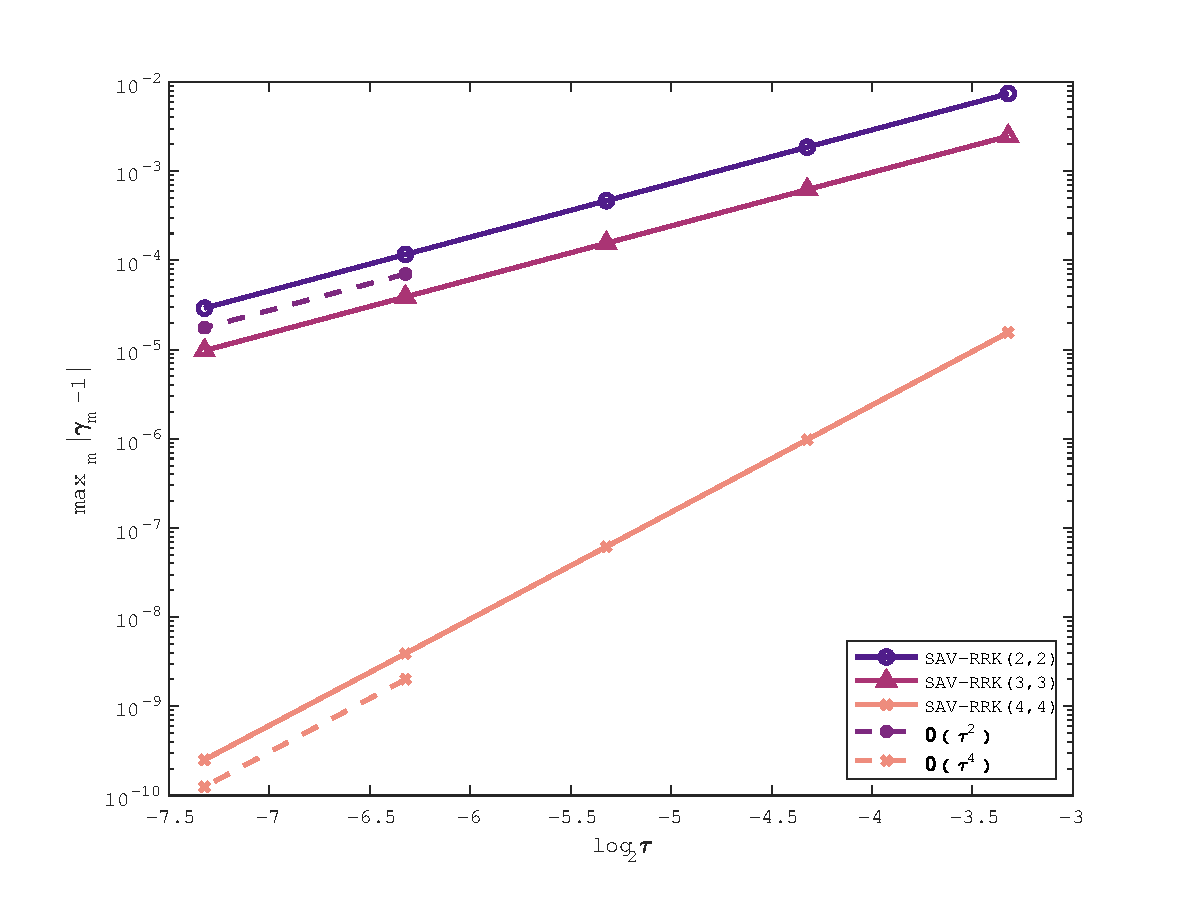
\includegraphics[width=0.5\textwidth]{./figures/exp1_r.eps}
	%\centerline{($b$) Spatial accuracy with $\tau = 10^{-3}.$}
	}\subfigure[$\max_m\left|S_m(1)\right|$]{ \centering
	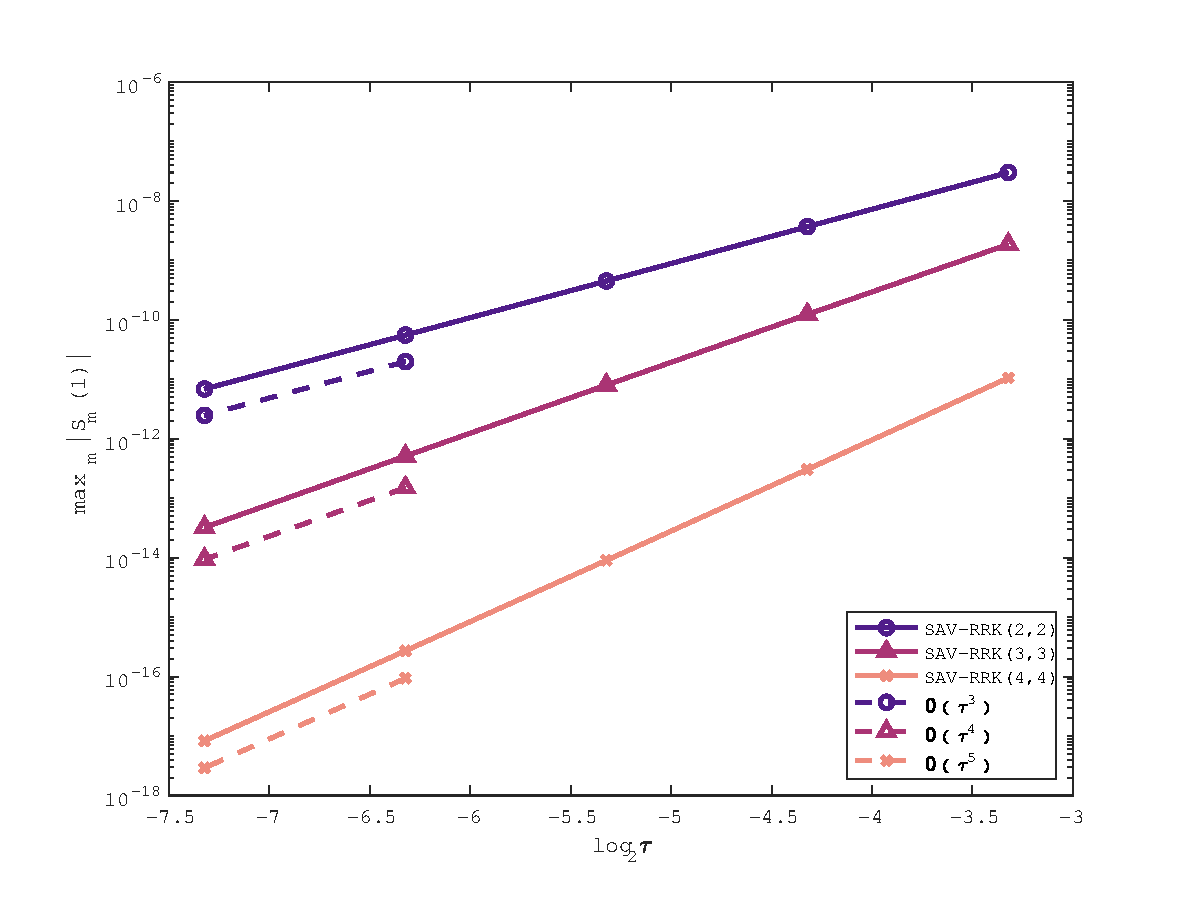
\includegraphics[width=0.5\textwidth]{./figures/exp1_s.eps}
	%\centerline{($a$) Temporal accuracy with $N=128.$}
	}
	% \caption{$\max_m\left|\gamma_m-1\right|$ and $\max_m\left|S_m(1)\right|$ for some relaxation methods in Example \ref{exp_SAVRRK:1}.}
	\caption{算例 \ref{exp_SAVRRK:1}的一些松弛格式所对应的$\max_m\left|\gamma_m-1\right|$ 和 $\max_m\left|S_m(1)\right|$.}
	\label{fig_SAVRRK:1}
	\end{center}
	\end{figure}
	使用SAV-RRK(4,4)方法,在长时间模拟($T=1000$)中,针对不同$\alpha$取值的相对能量误差如图 \ref{fig_SAVRRK:4}所示.
	这表明所提出的格式捕捉到了原始问题的保结构现象,并且其守恒性能明显优SAV方法\cite{chengConvergenceEnergyconservingScheme2022}和三层线性隐式差分法\cite{wangConservativeLinearizedDifference2015}.
	\begin{figure}[H]
		\begin{center}
		\subfigure[$\alpha=1.3$]{ \centering
		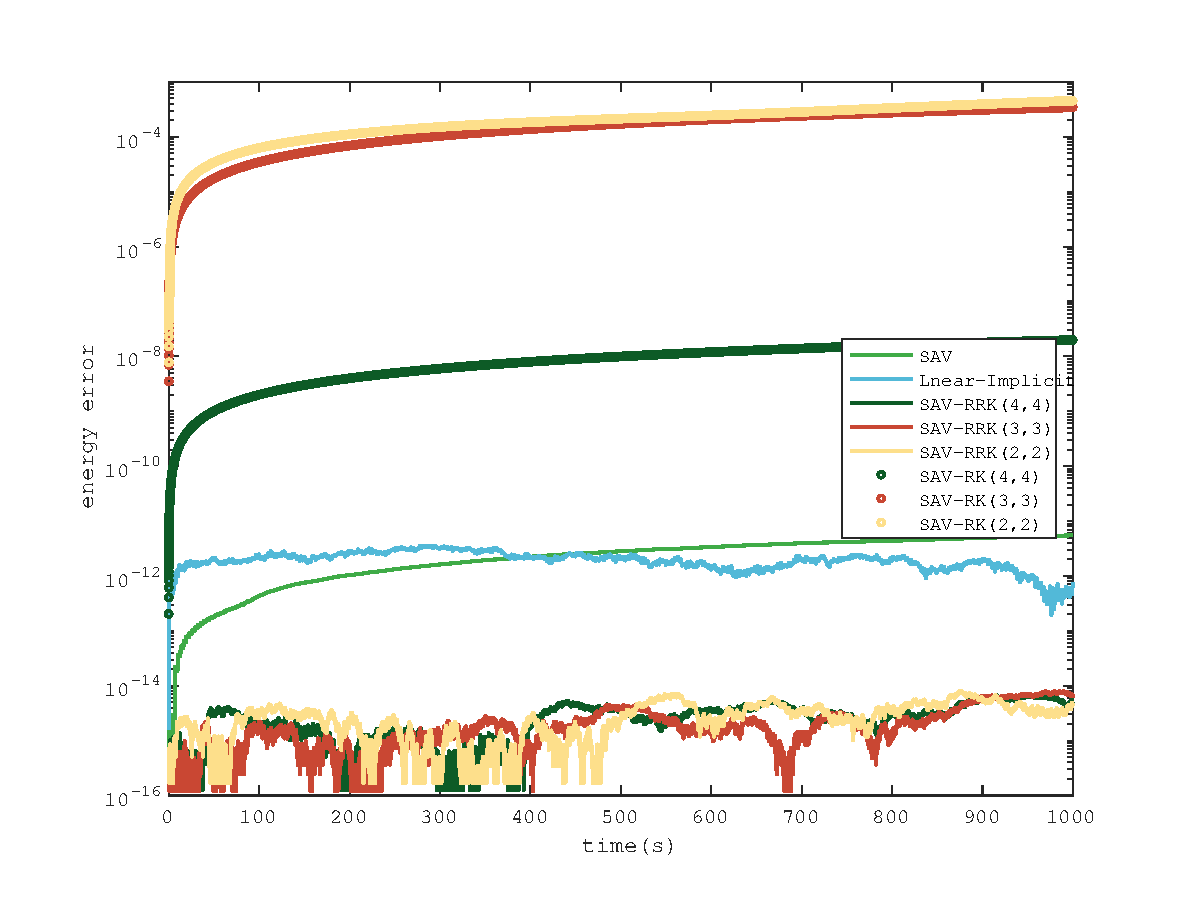
\includegraphics[width=0.5\textwidth]{./figures/exp1_energy3.eps}
		%\centerline{($b$) Spatial accuracy with $\tau = 10^{-3}.$}
		}\subfigure[$\alpha=1.6$]{ \centering
		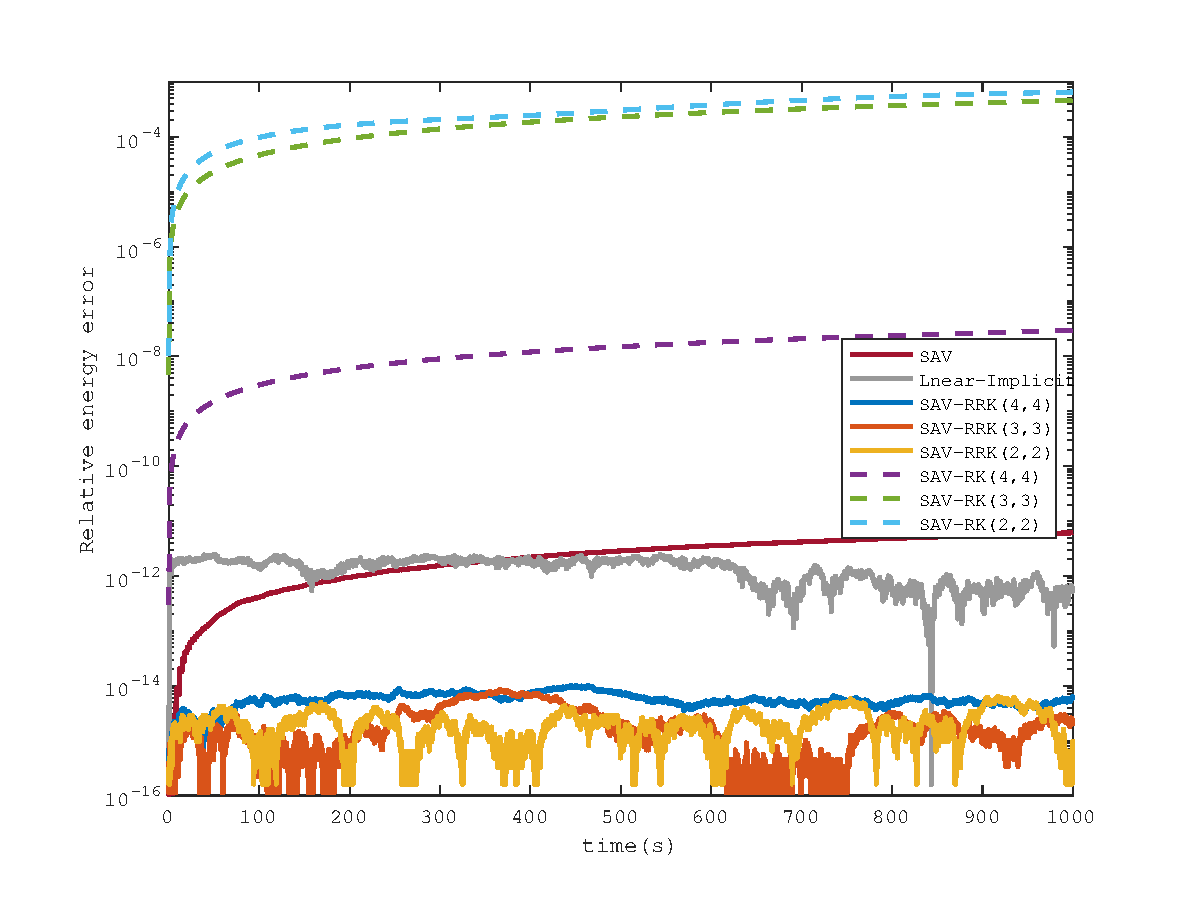
\includegraphics[width=0.5\textwidth]{./figures/exp1_energy6.eps}
		%\centerline{($a$) Temporal accuracy with $N=128.$}
		}\\
		\subfigure[$\alpha=1.9$]{ \centering
		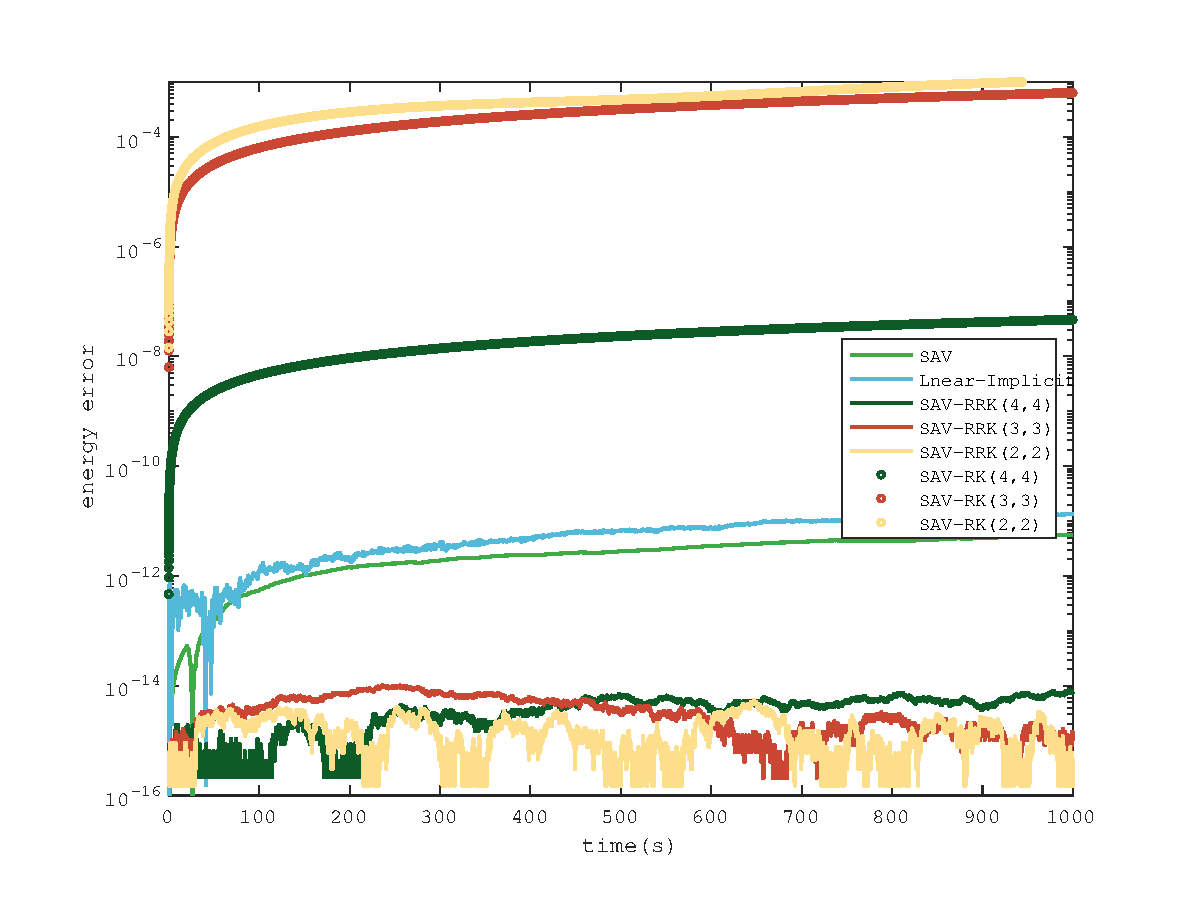
\includegraphics[width=0.5\textwidth]{./figures/exp1_energy9.eps}
		%\centerline{($b$) Spatial accuracy with $\tau = 10^{-3}.$}
		}\subfigure[$\alpha=2$]{ \centering
		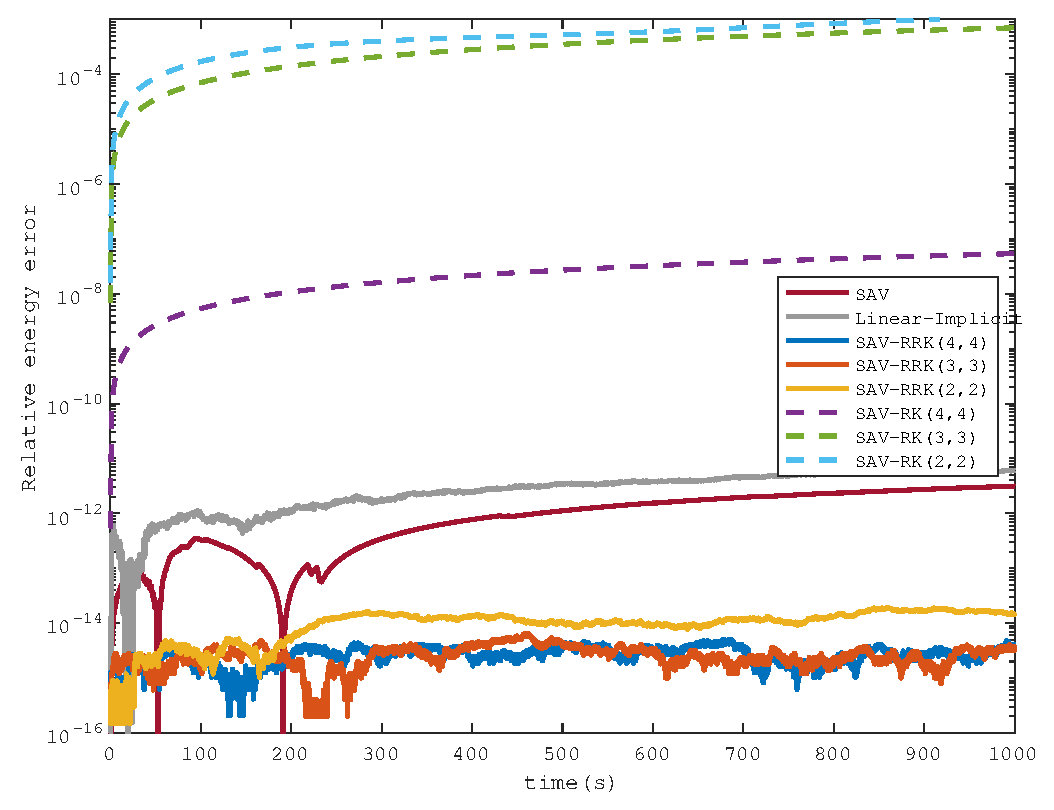
\includegraphics[width=0.5\textwidth]{./figures/exp1_energy2.eps}
		%\centerline{($a$) Temporal accuracy with $N=128.$}
		}
		% \caption{ Relative errors of energy with $N=32, \tau=0.01$ for different $\alpha$ in Example \ref{exp_SAVRRK:1}.}
		\caption{当 $N=32$,$\tau=0.01$ 时,算例 \ref{exp_SAVRRK:1} 取不同 $\alpha$ 对应的相对能量误差.}
		\label{fig_SAVRRK:4}
		\end{center}
		\end{figure}

	\begin{example}\label{exp_SAVRRK:2}
		考虑具有以下初值条件的二维 NFSWEs \eqref{eq_SAVRRK:1}-\eqref{eq_SAVRRK:3}
		\begin{equation*}
		u(x, y, 0)=\operatorname{sech}\left(x^2+y^2\right), u_t(x, y, 0)=\sin (x+y) \operatorname{sech}\left(-2\left(x^2+y^2\right)\right),(x, y, t) \in \Omega \times[0, T],
		\end{equation*}
		其中 $\Omega=[-5,5] \times[-5,5]$.
		\end{example}
			
		% 为了再次确认理论结果在二维情况下的适用性,使用算例 \ref{exp_SAVRRK:1} 中相同的参数($\alpha=1.5$ 和 $T=1$).
		设$\alpha=1.5$ 和 $T=1$,表 \ref{tab_SAVRRK:6-2} 和图 \ref{fig_SAVRRK:2-1} 分别展示了时间方向上的收敛阶以及对松弛因子 $\gamma$ 相关的理论验证.
		可以观察到,与 一维 算例\ref{exp_SAVRRK:1}不同, 在 二维 情况下,SAV-RRK(IDT) 方法未出现任何升阶现象.

\begin{table}[H]\scriptsize
\centering
\caption{当 $N=4, T = 1$ 时,算例 \ref{exp_SAVRRK:2} 在时间方向的误差和收敛阶}
% \caption{Numerical errors and convergence order in time for Example \ref{exp_SAVRRK:2} when $N=4, T = 1$.}
\begin{tabular}{lllllrlrlrlrlrl}
\toprule
\multicolumn{2}{l}{\multirow{2}[3]{*}{\textbf{RK(Stage,Order)}}} & \multicolumn{2}{l}{\multirow{2}[3]{*}{$\bm{\tau}$}} & \multicolumn{3}{c}{\textbf{SAV-RK}} &       & \multicolumn{3}{c}{\textbf{SAV-RRK}} &       & \multicolumn{3}{c}{\textbf{SAV-RRK(IDT)}} \\
\cmidrule{5-7}\cmidrule{9-11}\cmidrule{13-15}    \multicolumn{2}{l}{} & \multicolumn{2}{l}{} & \textbf{Error($\tau$)} &       & \textbf{order} &       & \textbf{Error($\tau$)} &       & \textbf{order} &       & \textbf{Error($\tau$)} &       & \textbf{order} \\
\hline
\multicolumn{2}{l}{\multirow{5}[0]{*}{\textbf{RK(2,2)}}} & \multicolumn{2}{l}{0.1} & 3.0217E-03 &       & -     &       & 3.0102E-03 &       & -     &       & 1.5692E-02 &       & - \\
\multicolumn{2}{l}{} & \multicolumn{2}{l}{0.05} & 7.4615E-04 &       & 2.0178  &       & 7.4702E-04 &       & 2.0106  &       & 9.6213E-03 &       & 0.7057  \\
\multicolumn{2}{l}{} & \multicolumn{2}{l}{0.025} & 1.8513E-04 &       & 2.0109  &       & 1.8587E-04 &       & 2.0069  &       & 5.2472E-03 &       & 0.8747  \\
\multicolumn{2}{l}{} & \multicolumn{2}{l}{0.0125} & 4.6090E-05 &       & 2.0060  &       & 4.6341E-05 &       & 2.0039  &       & 2.7312E-03 &       & 0.9420  \\
\multicolumn{2}{l}{} & \multicolumn{2}{l}{0.00625} & 1.1497E-05 &       & 2.0032  &       & 1.1569E-05 &       & 2.0021  &       & 1.3923E-03 &       & 0.9721  \\
\multicolumn{2}{l}{\multirow{5}[0]{*}{\textbf{RK(3,3)}}} & \multicolumn{2}{l}{0.1} & 1.2581E-04 &       & -     &       & 3.9379E-05 &       & -     &       & 3.2535E-03 &       & - \\
\multicolumn{2}{l}{} & \multicolumn{2}{l}{0.05} & 1.6180E-05 &       & 2.9589  &       & 5.5726E-06 &       & 2.8210  &       & 7.9304E-04 &       & 2.0365  \\
\multicolumn{2}{l}{} & \multicolumn{2}{l}{0.025} & 2.0532E-06 &       & 2.9783  &       & 7.4443E-07 &       & 2.9041  &       & 1.9546E-04 &       & 2.0205  \\
\multicolumn{2}{l}{} & \multicolumn{2}{l}{0.0125} & 2.5863E-07 &       & 2.9889  &       & 9.6210E-08 &       & 2.9519  &       & 4.8500E-05 &       & 2.0108  \\
\multicolumn{2}{l}{} & \multicolumn{2}{l}{0.00625} & 3.2454E-08 &       & 2.9944  &       & 1.2228E-08 &       & 2.9760  &       & 1.2078E-05 &       & 2.0056  \\
\multicolumn{2}{l}{\multirow{5}[1]{*}{\textbf{RK(4,4)}}} & \multicolumn{2}{l}{0.1} & 7.9185E-06 &       & -     &       & 8.0508E-06 &       & -     &       & 3.4013E-05 &       & - \\
\multicolumn{2}{l}{} & \multicolumn{2}{l}{0.05} & 4.9103E-07 &       & 4.0113  &       & 4.9644E-07 &       & 4.0194  &       & 3.3898E-06 &       & 3.3268  \\
\multicolumn{2}{l}{} & \multicolumn{2}{l}{0.025} & 3.0531E-08 &       & 4.0075  &       & 3.0805E-08 &       & 4.0104  &       & 3.6901E-07 &       & 3.1995  \\
\multicolumn{2}{l}{} & \multicolumn{2}{l}{0.0125} & 1.9026E-09 &       & 4.0042  &       & 1.9182E-09 &       & 4.0054  &       & 4.2681E-08 &       & 3.1120  \\
\multicolumn{2}{l}{} & \multicolumn{2}{l}{0.00625} & 1.1873E-10 &       & 4.0022  &       & 1.1966E-10 &       & 4.0027  &       & 5.1191E-09 &       & 3.0596  \\
\bottomrule
\end{tabular}%
\label{tab_SAVRRK:6-2}%
\end{table}%
	
\begin{figure}[H]
\begin{center}
\subfigure[$\max_m\left|\gamma_m-1\right|$]{ \centering
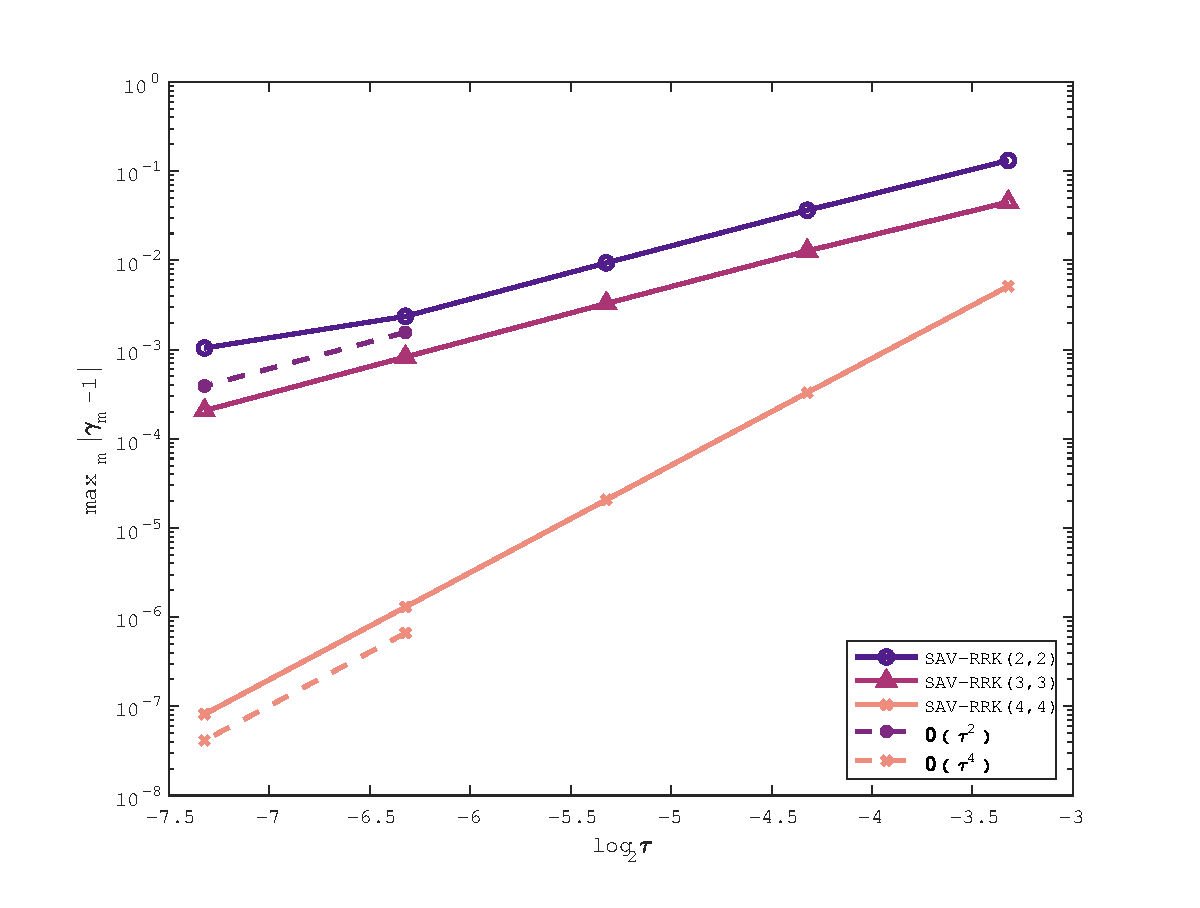
\includegraphics[width=0.5\textwidth]{./figures/exp2_r.eps}
%\centerline{($b$) Spatial accuracy with $\tau = 10^{-3}.$}
}\subfigure[$\max_m\left|S_m(1)\right|$]{ \centering
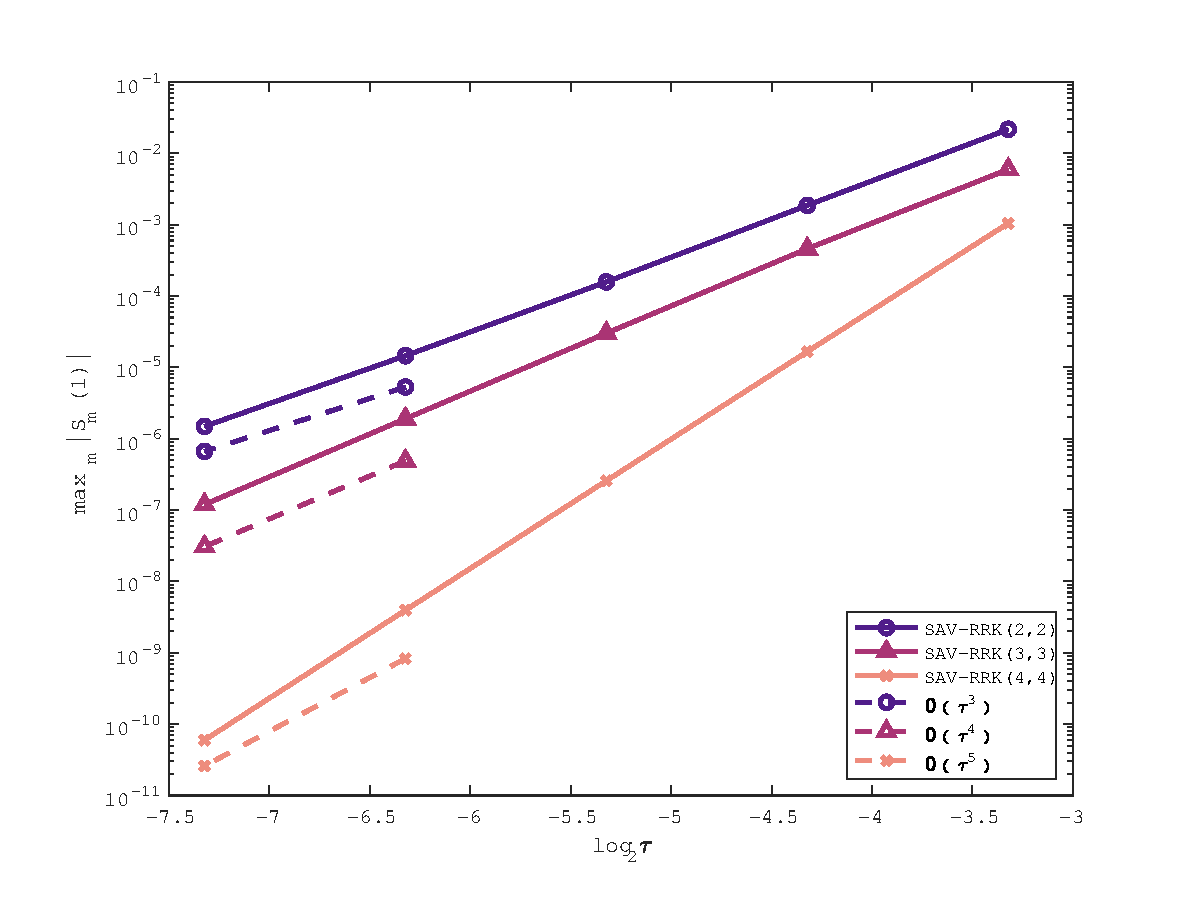
\includegraphics[width=0.5\textwidth]{./figures/exp2_s.eps}
%\centerline{($a$) Temporal accuracy with $N=128.$}
}
% \caption{$\max _m\left|\gamma_m-1\right|$ and $\max_m\left|S_m(1)\right|$ for some relaxation (RT) methods in Example \ref{exp_SAVRRK:2}.}
\caption{算例 \ref{exp_SAVRRK:2}的一些松弛格式所对应的$\max_m\left|\gamma_m-1\right|$ 和 $\max_m\left|S_m(1)\right|$.}
\label{fig_SAVRRK:2-1}
\end{center}
\end{figure}
为了展示所提方法在保持能量守恒方面的有效性,在图 \ref{fig_SAVRRK:2-4} 中绘制了取不同的$\alpha$时,使用 SAV-RRK(4,4) 方法进行长时间模拟($T=100$)的相对能量误差.
结果显示, 所提出的方法可以在离散层面上精确地保持能量,且其能量守恒性能显著优于 SAV 方法 \cite{chengConvergenceEnergyconservingScheme2022}.
\begin{figure}[H]
	\begin{center}
	\subfigure[$\alpha=1.3$]{ \centering
	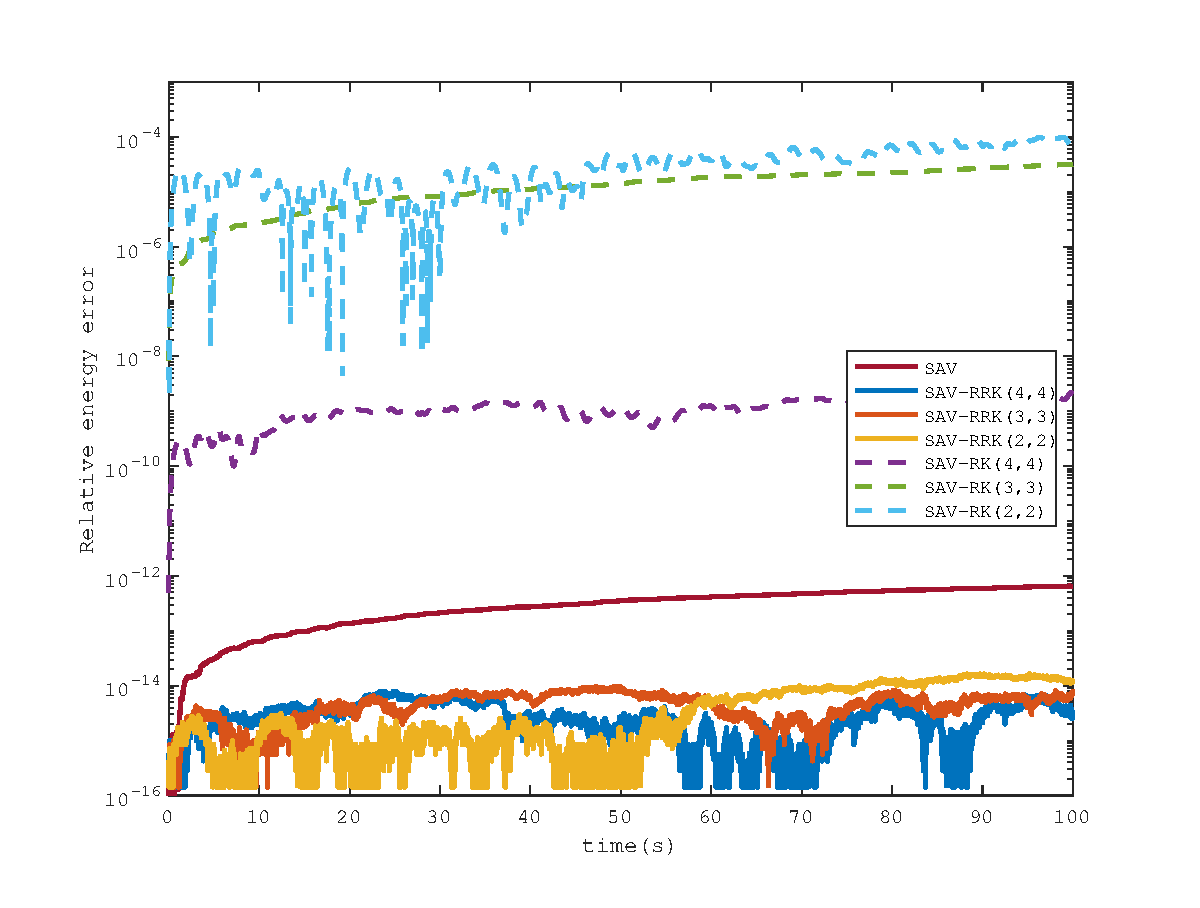
\includegraphics[width=0.5\textwidth]{./figures/exp2_energy3.eps}
	%\centerline{($b$) Spatial accuracy with $\tau = 10^{-3}.$}
	}\subfigure[$\alpha=1.6$]{ \centering
	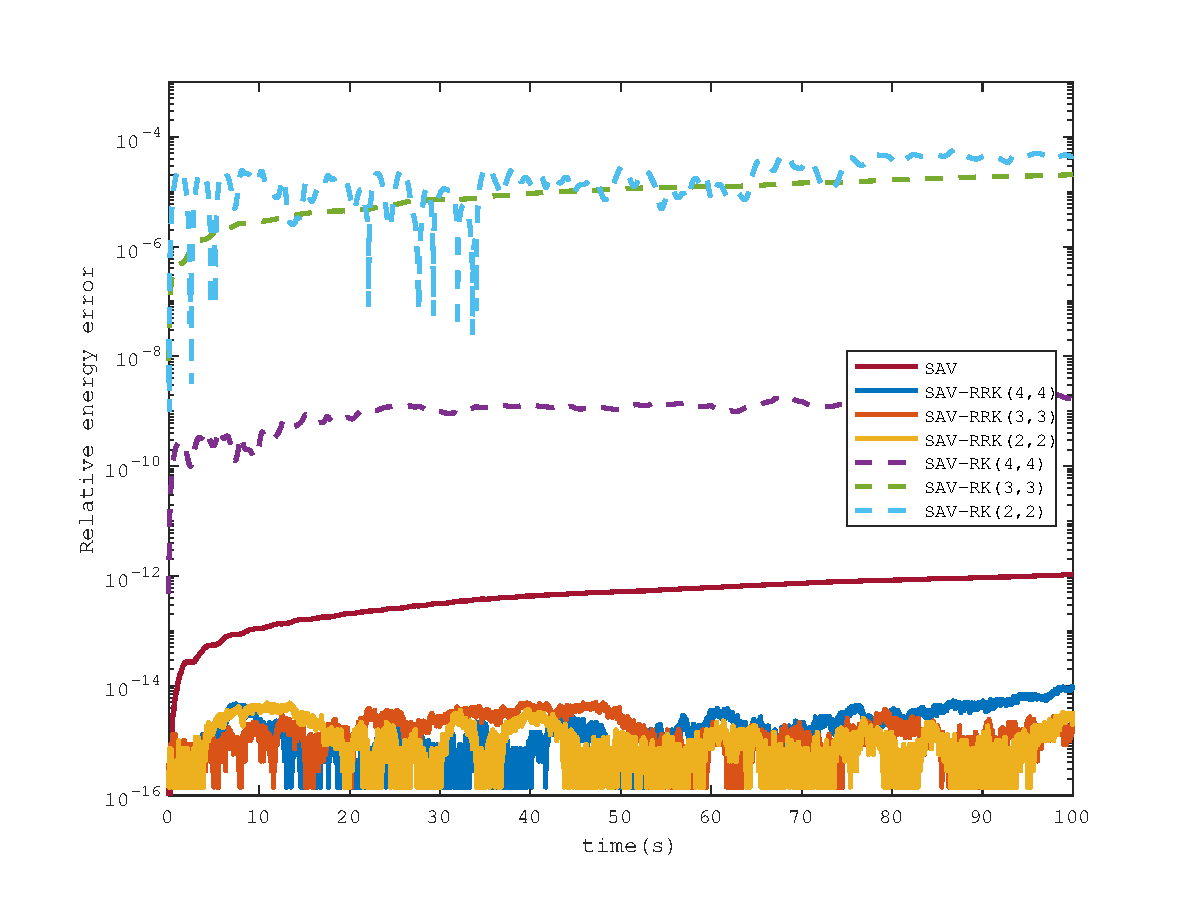
\includegraphics[width=0.5\textwidth]{./figures/exp2_energy6.eps}
	%\centerline{($a$) Temporal accuracy with $N=128.$}
	}\\
	\subfigure[$\alpha=1.9$]{ \centering
	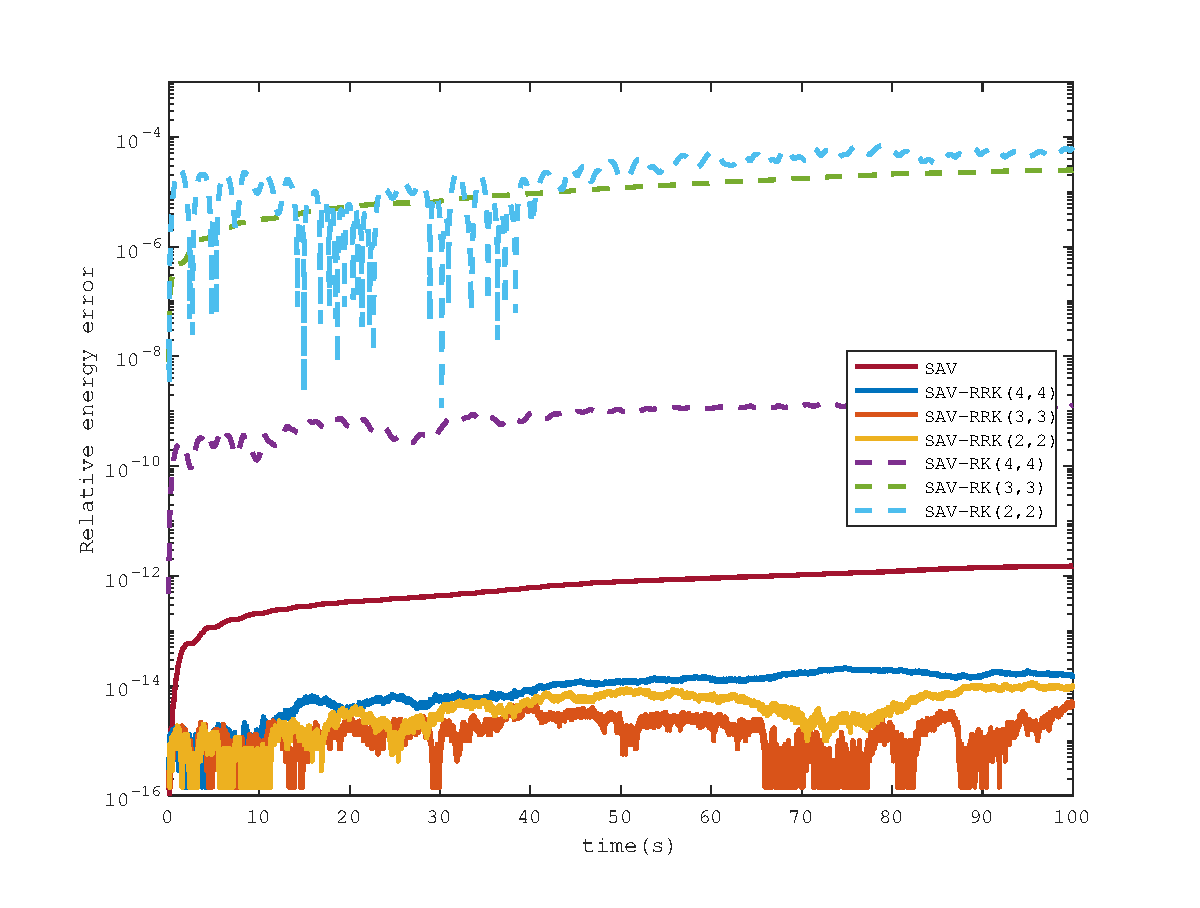
\includegraphics[width=0.5\textwidth]{./figures/exp2_energy9.eps}
	%\centerline{($b$) Spatial accuracy with $\tau = 10^{-3}.$}
	}\subfigure[$\alpha=2$]{ \centering
	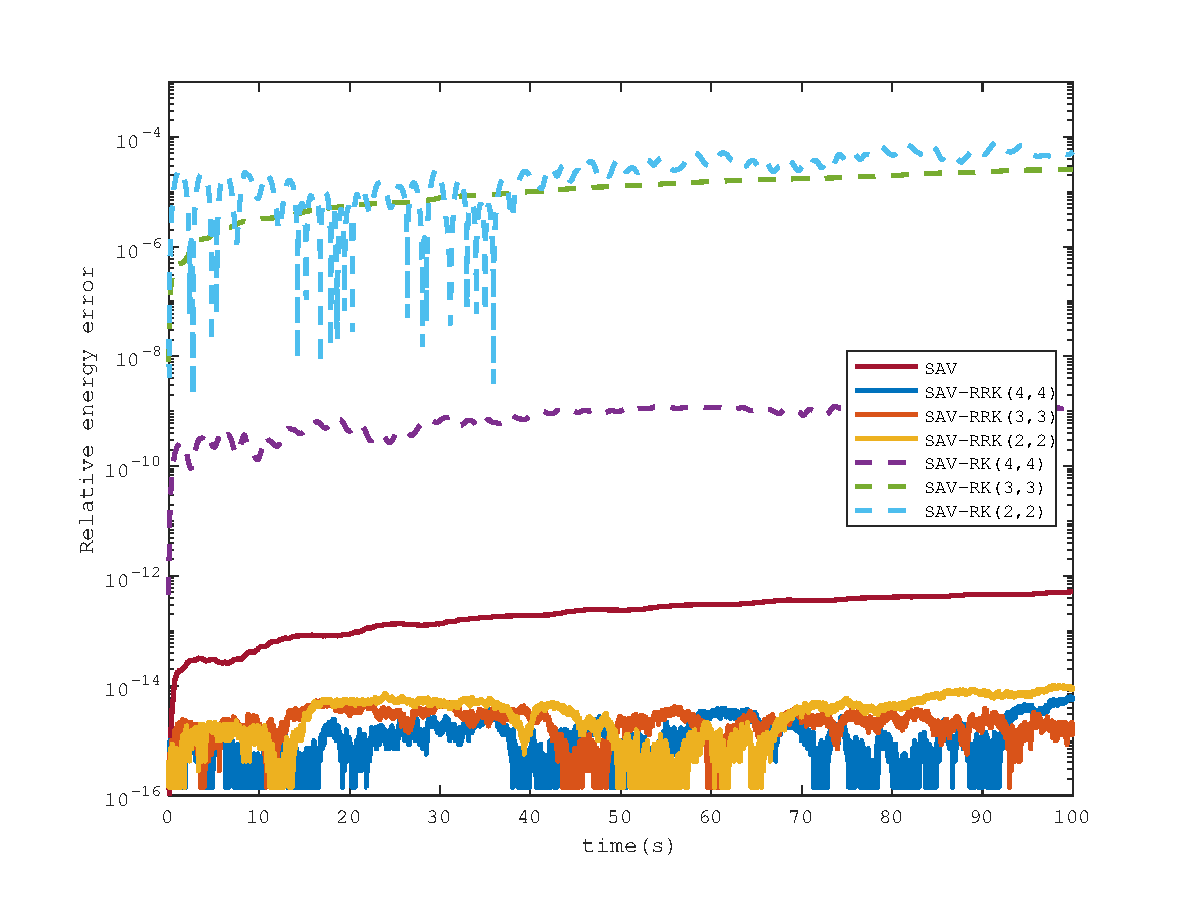
\includegraphics[width=0.5\textwidth]{./figures/exp2_energy2.eps}
	%\centerline{($a$) Temporal accuracy with $N=128.$}
	}
	% \caption{ Relative errors of energy with $N=4, \tau=0.01$ for different $\alpha$ in Example \ref{exp_SAVRRK:2}.}
	\caption{当 $N=4, \tau=0.01$ 时,算例 \ref{exp_SAVRRK:2} 取不同 $\alpha$ 对应的相对能量误差.}
	\label{fig_SAVRRK:2-4}
	\end{center}
	\end{figure}
	
	\begin{example}\label{exp_SAVRRK:3}
		考虑二维非线性分数阶波动方程\cite{wangUnconditionalEnergyDissipation2021} 
		\begin{equation}
		\begin{cases}
		& u_{t t}+(-\Delta)^{\frac{\alpha}{2}} u+F^{\prime}(u)=0,(x, y, t) \in \Omega \times(0, T],\\
		& u(x, y, 0)=\frac{1}{2} \arctan \left(\exp \left(-\sqrt{x^2+y^2}\right)\right), u_t(x, y, 0)=0,
		\end{cases}
		\end{equation}
		其中 $\Omega=(-10,10) \times(-10,10)$,势能 $F(u)=u^2\left(\frac{1}{4} u^2-\frac{1}{2}\right)$.
		\end{example}
		
		取 $\alpha=1.5$ 和 $T=1$,表 \ref{tab_SAVRRK:6-3} 展示了标准 SAV-RK、SAV-RRK(RT) 和 SAV-RRK(IDT) 方法在时间方向上的误差和收敛阶.
		此外,图 \ref{fig_SAVRRK:3-4} 展示了长时间模拟 ($T=100$) 的相对能量误差,这些数据是通过 SAV-RRK(4,4) 方法计算获得.
		结果表明,本章所提出的方法对非线性分数阶波动方程也是有效的.
		
\begin{table}[H]\scriptsize
\centering
% \caption{Numerical errors and convergence order in time for Example \ref{exp_SAVRRK:3} when $N=4, T = 1$.}
\caption{当 $N=4, T = 1$ 时,算例 \ref{exp_SAVRRK:3} 在时间方向的误差和收敛阶}
\begin{tabular}{lllllrlrlrlrlrl}
\toprule
\multicolumn{2}{l}{\multirow{2}[3]{*}{\textbf{RK(Stage,Order)}}} & \multicolumn{2}{l}{\multirow{2}[3]{*}{$\bm{\tau}$}} & \multicolumn{3}{c}{\textbf{SAV-RK}} &       & \multicolumn{3}{c}{\textbf{SAV-RRK(RT)}} &       & \multicolumn{3}{c}{\textbf{SAV-RRK(IDT)}} \\
\cmidrule{5-7}\cmidrule{9-11}\cmidrule{13-15}    \multicolumn{2}{l}{} & \multicolumn{2}{l}{} & \textbf{Error($\tau$)} &       & \textbf{order} &       & \textbf{Error($\tau$)} &       & \textbf{order} &       & \textbf{Error($\tau$)} &       & \textbf{order} \\
\hline
\multicolumn{2}{l}{\multirow{5}[0]{*}{\textbf{RK(2,2)}}} & \multicolumn{2}{l}{0.1} & 1.3395E-03 &       & -     &       & 3.3870E-03 &       & -     &       & 2.1470E-02 &       & - \\
\multicolumn{2}{l}{} & \multicolumn{2}{l}{0.05} & 3.4360E-04 &       & 1.9628  &       & 8.1480E-04 &       & 2.0555  &       & 1.0960E-02 &       & 0.9701  \\
\multicolumn{2}{l}{} & \multicolumn{2}{l}{0.025} & 8.6945E-05 &       & 1.9826  &       & 1.9951E-04 &       & 2.0300  &       & 5.5113E-03 &       & 0.9918  \\
\multicolumn{2}{l}{} & \multicolumn{2}{l}{0.0125} & 2.1865E-05 &       & 1.9915  &       & 4.9347E-05 &       & 2.0154  &       & 2.7600E-03 &       & 0.9977  \\
\multicolumn{2}{l}{} & \multicolumn{2}{l}{0.00625} & 5.4823E-06 &       & 1.9958  &       & 1.2270E-05 &       & 2.0078  &       & 1.3807E-03 &       & 0.9993  \\
\multicolumn{2}{l}{\multirow{5}[0]{*}{\textbf{RK(3,3)}}} & \multicolumn{2}{l}{0.1} & 3.5168E-05 &       & -     &       & 4.3927E-05 &       & -     &       & 3.8213E-04 &       & - \\
\multicolumn{2}{l}{} & \multicolumn{2}{l}{0.05} & 4.3533E-06 &       & 3.0141  &       & 5.4825E-06 &       & 3.0022  &       & 8.0473E-05 &       & 2.2475  \\
\multicolumn{2}{l}{} & \multicolumn{2}{l}{0.025} & 5.3902E-07 &       & 3.0137  &       & 6.8378E-07 &       & 3.0032  &       & 1.8560E-05 &       & 2.1163  \\
\multicolumn{2}{l}{} & \multicolumn{2}{l}{0.0125} & 6.7058E-08 &       & 3.0068  &       & 8.5344E-08 &       & 3.0022  &       & 4.4475E-06 &       & 2.0611  \\
\multicolumn{2}{l}{} & \multicolumn{2}{l}{0.00625} & 8.3615E-09 &       & 3.0036  &       & 1.0659E-08 &       & 3.0012  &       & 1.0883E-06 &       & 2.0309  \\
\multicolumn{2}{l}{\multirow{5}[1]{*}{\textbf{RK(4,4)}}} & \multicolumn{2}{l}{0.1} & 5.3561E-07 &       & -     &       & 3.2716E-06 &       & -     &       & 3.7745E-05 &       & - \\
\multicolumn{2}{l}{} & \multicolumn{2}{l}{0.05} & 3.6438E-08 &       & 3.8777  &       & 2.0654E-07 &       & 3.9855  &       & 4.8050E-06 &       & 2.9737  \\
\multicolumn{2}{l}{} & \multicolumn{2}{l}{0.025} & 2.3735E-09 &       & 3.9403  &       & 1.2898E-08 &       & 4.0012  &       & 6.0237E-07 &       & 2.9958  \\
\multicolumn{2}{l}{} & \multicolumn{2}{l}{0.0125} & 1.5146E-10 &       & 3.9700  &       & 8.0476E-10 &       & 4.0024  &       & 7.5303E-08 &       & 2.9999  \\
\multicolumn{2}{l}{} & \multicolumn{2}{l}{0.00625} & 9.5636E-12 &       & 3.9853  &       & 5.0241E-11 &       & 4.0016  &       & 9.4105E-09 &       & 3.0004  \\
\bottomrule
\end{tabular}%
\label{tab_SAVRRK:6-3}%
\end{table}%
\vspace{-10mm}

\begin{figure}[H]
\begin{center}
\subfigure[$\alpha=1.3$]{ \centering
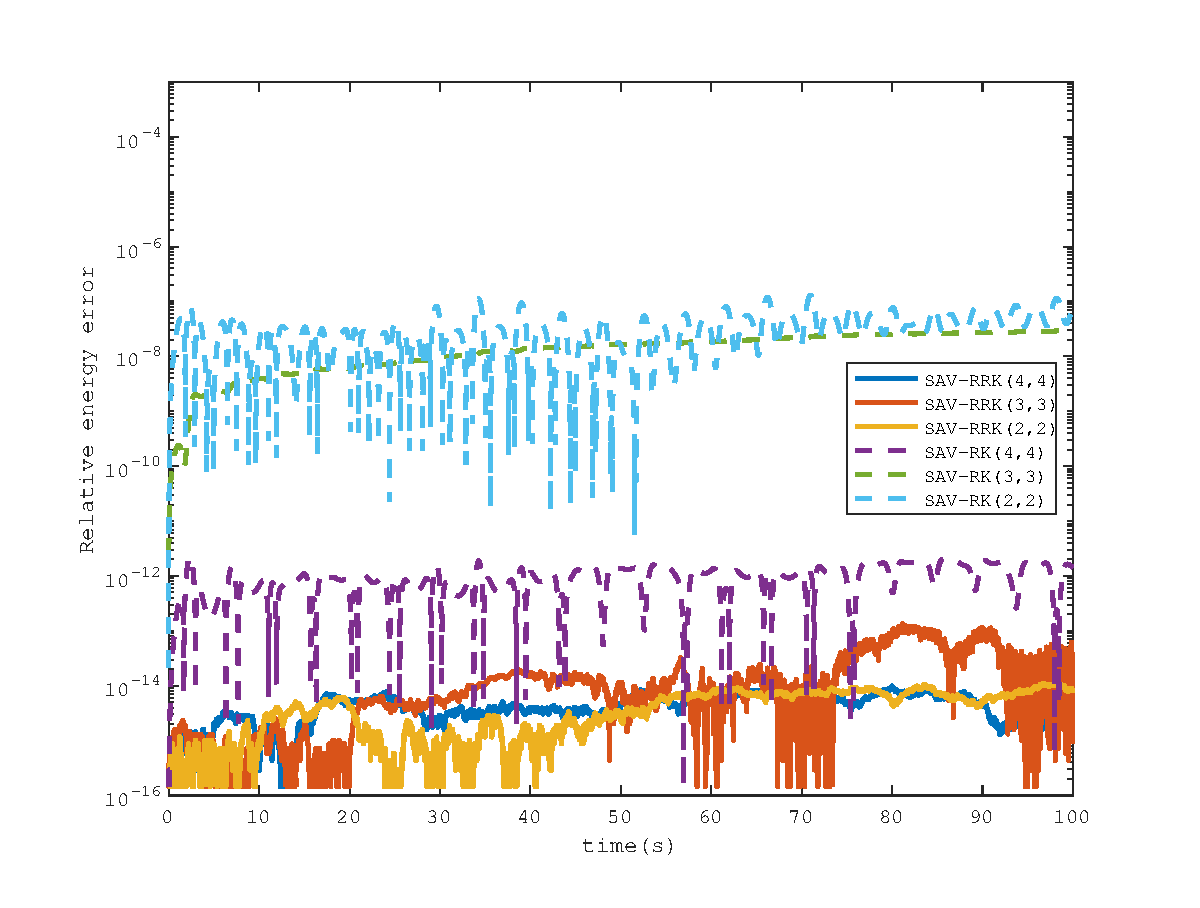
\includegraphics[width=0.5\textwidth]{./figures/exp3_energy3.eps}
%\centerline{($b$) Spatial accuracy with $\tau = 10^{-3}.$}
}\subfigure[$\alpha=1.6$]{ \centering
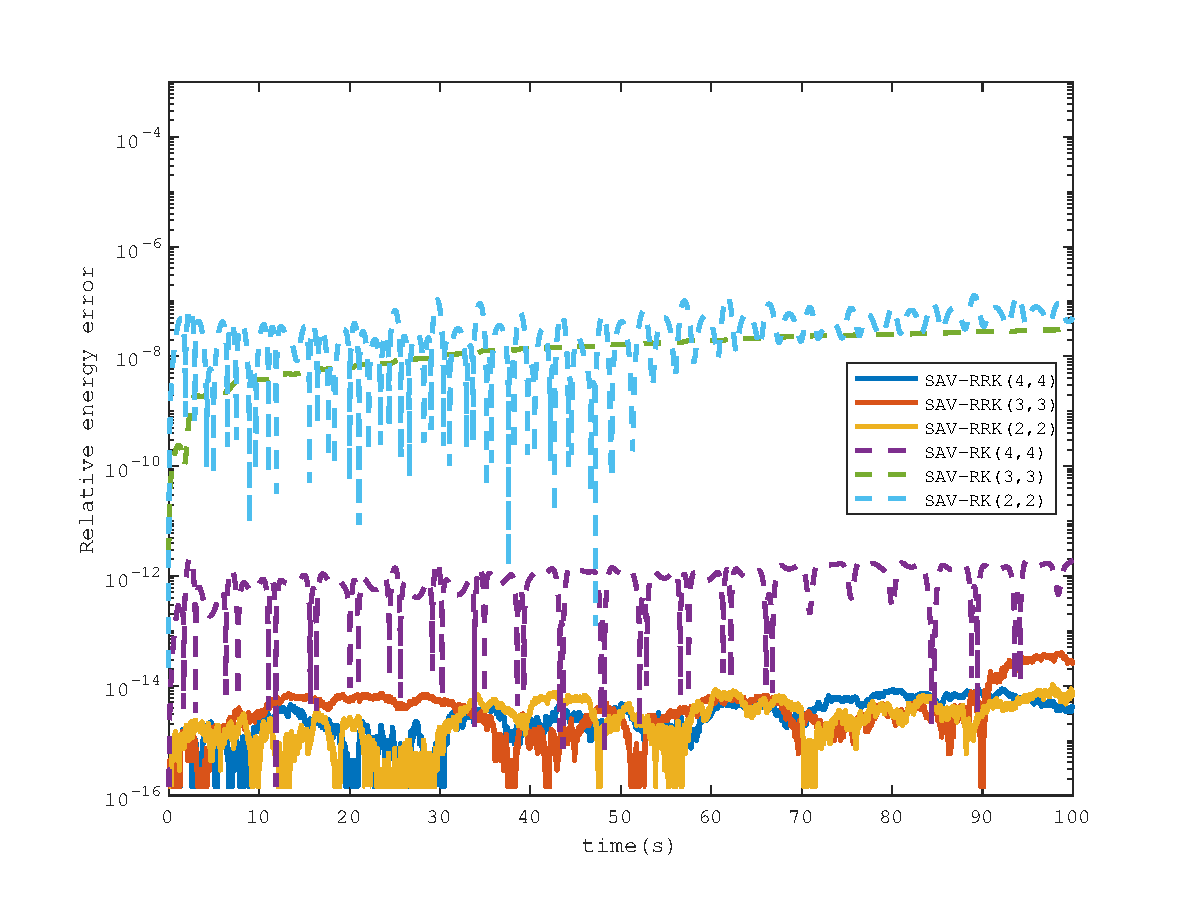
\includegraphics[width=0.5\textwidth]{./figures/exp3_energy6.eps}
%\centerline{($a$) Temporal accuracy with $N=128.$}
}\\
\subfigure[$\alpha=1.9$]{ \centering
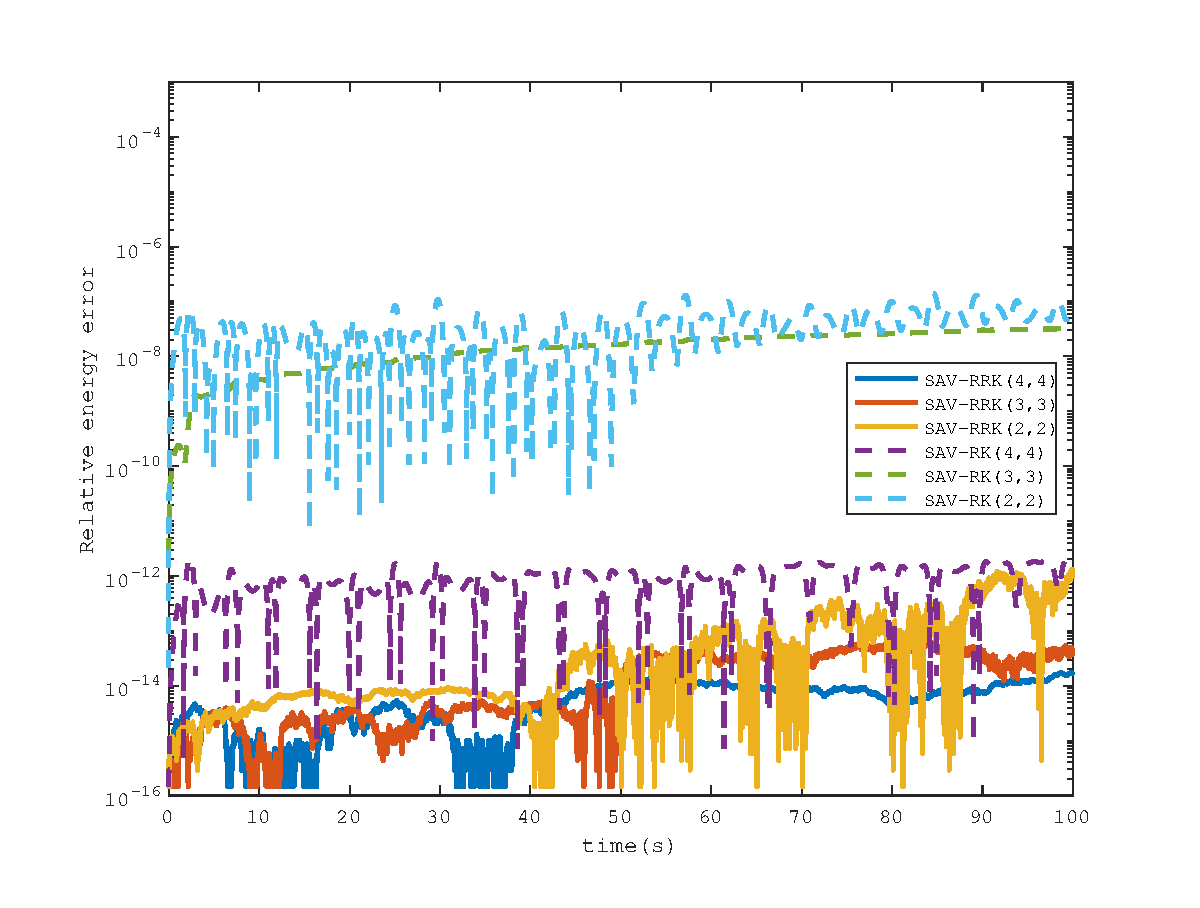
\includegraphics[width=0.5\textwidth]{./figures/exp3_energy9.eps}
%\centerline{($b$) Spatial accuracy with $\tau = 10^{-3}.$}
}\subfigure[$\alpha=2$]{ \centering
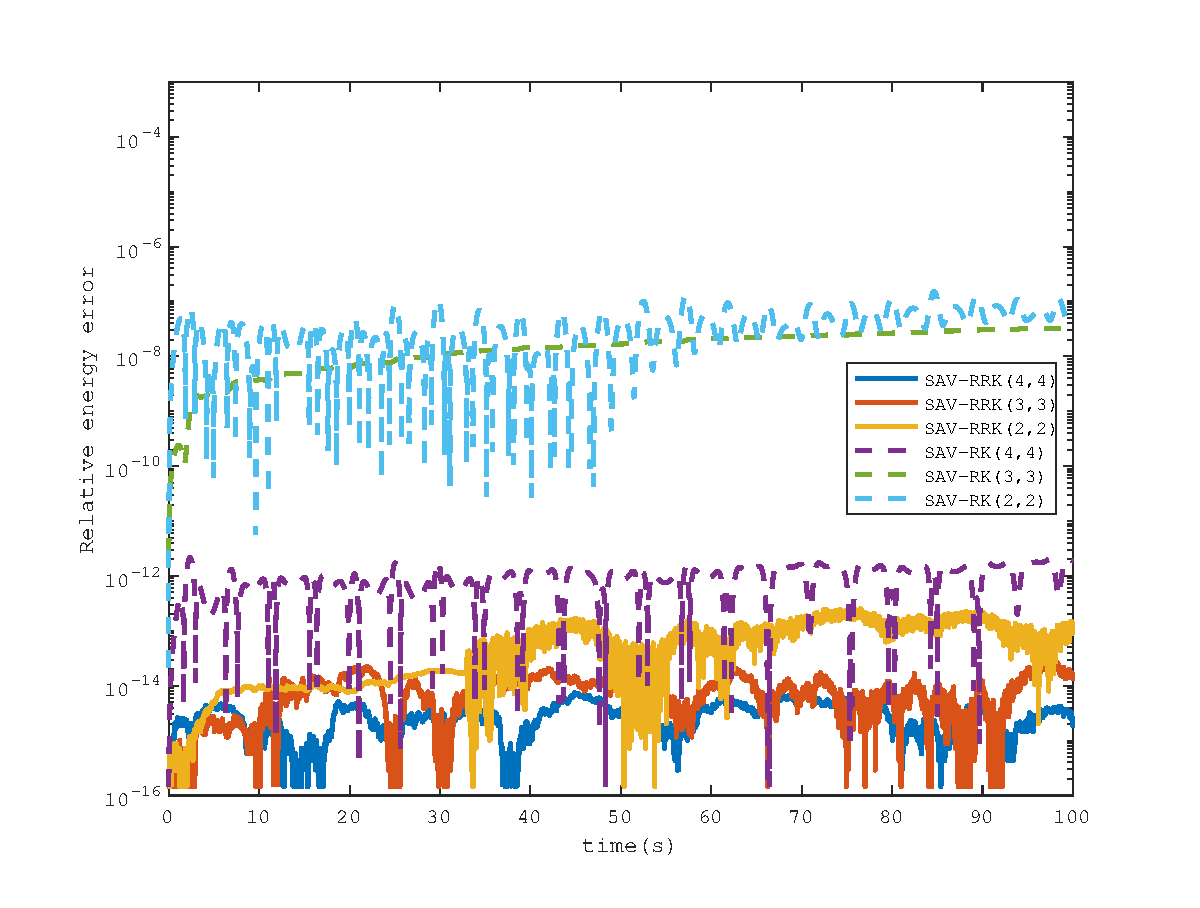
\includegraphics[width=0.5\textwidth]{./figures/exp3_energy2.eps}
%\centerline{($a$) Temporal accuracy with $N=128.$}
}
% \caption{ Relative errors of energy with $N=4, \tau=0.01$ for different $\alpha$ in Example \ref{exp_SAVRRK:3}.}
\caption{当 $N=4, \tau=0.01$ 时,算例 \ref{exp_SAVRRK:3} 取不同 $\alpha$ 对应的相对能量误差.}
\label{fig_SAVRRK:3-4}
\end{center}
\end{figure}

\begin{example}\label{exp_SAVRRK:4}
考虑二维分数阶Klein-Gordon-Schr{\"o}dinger方程\cite{fuStructurepreservingAlgorithmsTwodimensional2020}
\begin{equation}
\begin{cases}
\mathrm{i} \partial_t u-\frac{1}{2}(-\Delta)^{\frac{\alpha}{2}} u+u \phi=0,(x, y, t) \in \Omega \times(0, T],\\
\partial_{t t} \phi+(-\Delta)^{\frac{\beta}{2}} \phi+\phi-|u|^2=0, (x, y, t) \in \Omega \times(0, T],
\end{cases}
\end{equation}
初值条件为
\begin{equation}
	\begin{aligned}
		u(x, y, 0)&=(1+\mathrm{i}) \exp \left(-|\boldsymbol{x}|^2\right),~~\phi(x, y, 0)=\operatorname{sech}\left(|\boldsymbol{x}|^2\right),\\
		\partial_t \phi(x, y, 0)&=\sin (x+y) \operatorname{sech}\left(-2|\boldsymbol{x}|^2\right),
	\end{aligned}
\end{equation}
其中 $\Omega=[-10,10] \times[-10,10]$.
\end{example}

与前面的算例类似,表 \ref{tab_SAVRRK:6-4} 列出了 $\alpha=\beta=1.5$ 时的一些数值误差和时间方向收敛阶.


\begin{table}[H]\scriptsize
\centering
% \caption{Numerical errors and convergence order in time for Example \ref{exp_SAVRRK:4} when $N=4, T = 1$.}
\caption{当 $N=4, T = 1$ 时,算例 \ref{exp_SAVRRK:4} 在时间方向的误差和收敛阶}
\begin{tabular}{lllllrlrlrlrlrl}
\toprule
\multicolumn{2}{l}{\multirow{2}[3]{*}{\textbf{RK(Stage,Order)}}} & \multicolumn{2}{l}{\multirow{2}[3]{*}{$\bm{\tau}$}} & \multicolumn{3}{c}{\textbf{SAV-RK}} &       & \multicolumn{3}{c}{\textbf{SAV-RRK(RT)}} &       & \multicolumn{3}{c}{\textbf{SAV-RRK(IDT)}} \\
\cmidrule{5-7}\cmidrule{9-11}\cmidrule{13-15}    \multicolumn{2}{l}{} & \multicolumn{2}{l}{} & \textbf{Error($\tau$)} &       & \textbf{order} &       & \textbf{Error($\tau$)} &       & \textbf{order} &       & \textbf{Error($\tau$)} &       & \textbf{order} \\
\hline
\multicolumn{2}{l}{\multirow{5}[0]{*}{\textbf{RK(2,2)}}} & \multicolumn{2}{l}{0.1} & 1.1875E-03 &       & -     &       & 1.8837E-03 &       & -     &       & 9.5325E-03 &       & - \\
\multicolumn{2}{l}{} & \multicolumn{2}{l}{0.05} & 2.7648E-04 &       & 2.1026  &       & 5.0394E-04 &       & 1.9023  &       & 6.7134E-03 &       & 0.5058  \\
\multicolumn{2}{l}{} & \multicolumn{2}{l}{0.025} & 6.6514E-05 &       & 2.0555  &       & 1.3036E-04 &       & 1.9508  &       & 3.8805E-03 &       & 0.7908  \\
\multicolumn{2}{l}{} & \multicolumn{2}{l}{0.0125} & 1.6300E-05 &       & 2.0288  &       & 3.3151E-05 &       & 1.9754  &       & 2.0757E-03 &       & 0.9026  \\
\multicolumn{2}{l}{} & \multicolumn{2}{l}{0.00625} & 4.0339E-06 &       & 2.0146  &       & 8.3587E-06 &       & 1.9877  &       & 1.0723E-03 &       & 0.9529  \\
\multicolumn{2}{l}{\multirow{5}[0]{*}{\textbf{RK(3,3)}}} & \multicolumn{2}{l}{0.1} & 8.7748E-05 &       & -     &       & 1.9567E-04 &       & -     &       & 3.1789E-03 &       & - \\
\multicolumn{2}{l}{} & \multicolumn{2}{l}{0.05} & 1.1471E-05 &       & 2.9354  &       & 2.4630E-05 &       & 2.9900  &       & 8.2646E-04 &       & 1.9435  \\
\multicolumn{2}{l}{} & \multicolumn{2}{l}{0.025} & 1.4684E-06 &       & 2.9657  &       & 3.0916E-06 &       & 2.9940  &       & 2.1079E-04 &       & 1.9712  \\
\multicolumn{2}{l}{} & \multicolumn{2}{l}{0.0125} & 1.8580E-07 &       & 2.9824  &       & 3.8731E-07 &       & 2.9968  &       & 5.3231E-05 &       & 1.9854  \\
\multicolumn{2}{l}{} & \multicolumn{2}{l}{0.00625} & 2.3370E-08 &       & 2.9911  &       & 4.8471E-08 &       & 2.9983  &       & 1.3375E-05 &       & 1.9927  \\
\multicolumn{2}{l}{\multirow{5}[1]{*}{\textbf{RK(4,4)}}} & \multicolumn{2}{l}{0.1} & 3.0741E-06 &       & -     &       & 4.0627E-06 &       & -     &       & 1.0278E-04 &       & - \\
\multicolumn{2}{l}{} & \multicolumn{2}{l}{0.05} & 1.9959E-07 &       & 3.9450  &       & 2.6020E-07 &       & 3.9647  &       & 1.3195E-05 &       & 2.9615  \\
\multicolumn{2}{l}{} & \multicolumn{2}{l}{0.025} & 1.2698E-08 &       & 3.9744  &       & 1.6461E-08 &       & 3.9825  &       & 1.6711E-06 &       & 2.9811  \\
\multicolumn{2}{l}{} & \multicolumn{2}{l}{0.0125} & 8.0044E-10 &       & 3.9876  &       & 1.0350E-09 &       & 3.9913  &       & 2.1024E-07 &       & 2.9906  \\
\multicolumn{2}{l}{} & \multicolumn{2}{l}{0.00625} & 5.0238E-11 &       & 3.9939  &       & 6.4882E-11 &       & 3.9957  &       & 2.6365E-08 &       & 2.9953  \\
\bottomrule
\end{tabular}%
\label{tab_SAVRRK:6-4}%
\end{table}%

此外,使用不同 $\alpha$ 和 $\beta$ 进行长时间模拟($T=100$)的相对能量如图 \ref{fig_SAVRRK:3-5} 所示.

\begin{figure}[H]
\begin{center}
\subfigure[$\alpha,\beta=1.3$]{ \centering
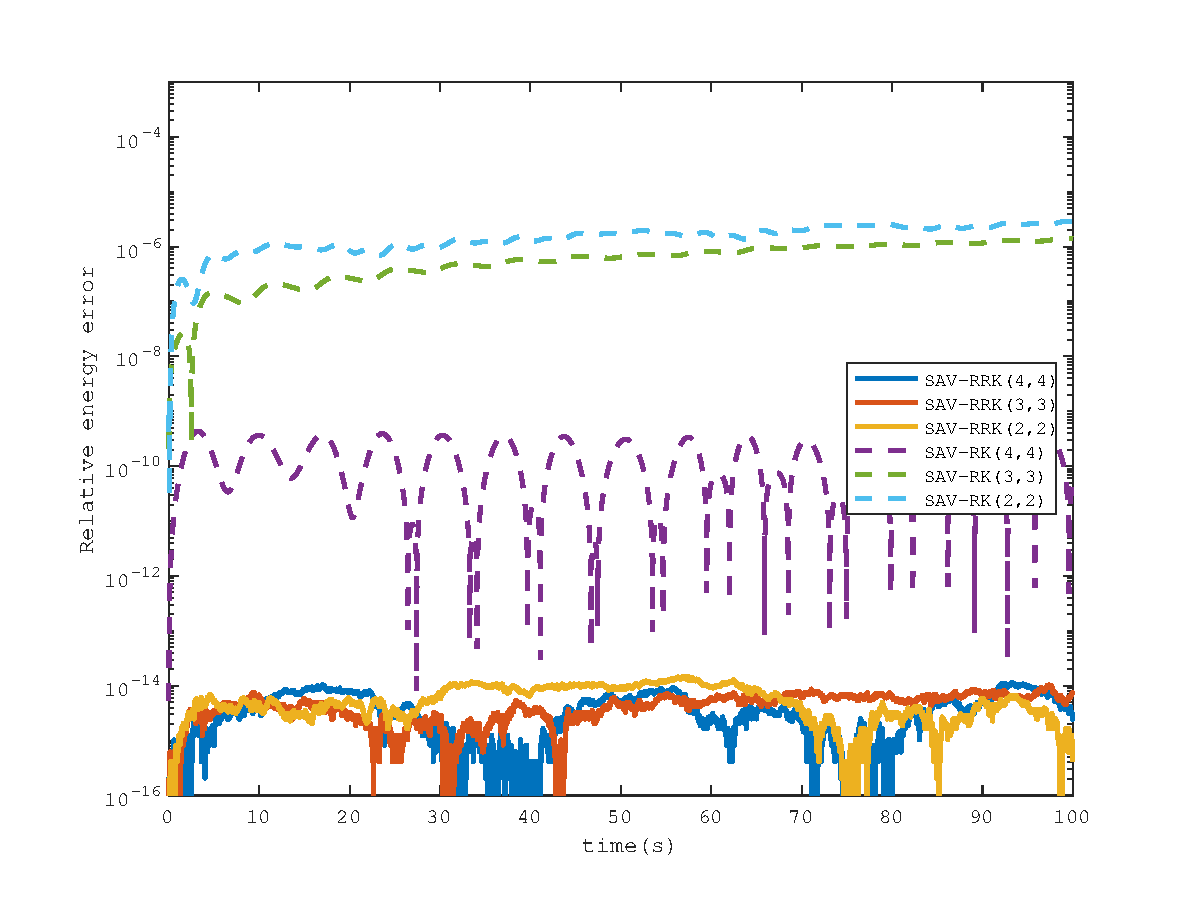
\includegraphics[width=0.5\textwidth]{./figures/exp4_energy3.eps}
%\centerline{($b$) Spatial accuracy with $\tau = 10^{-3}.$}
}\subfigure[$\alpha,\beta=1.6$]{ \centering
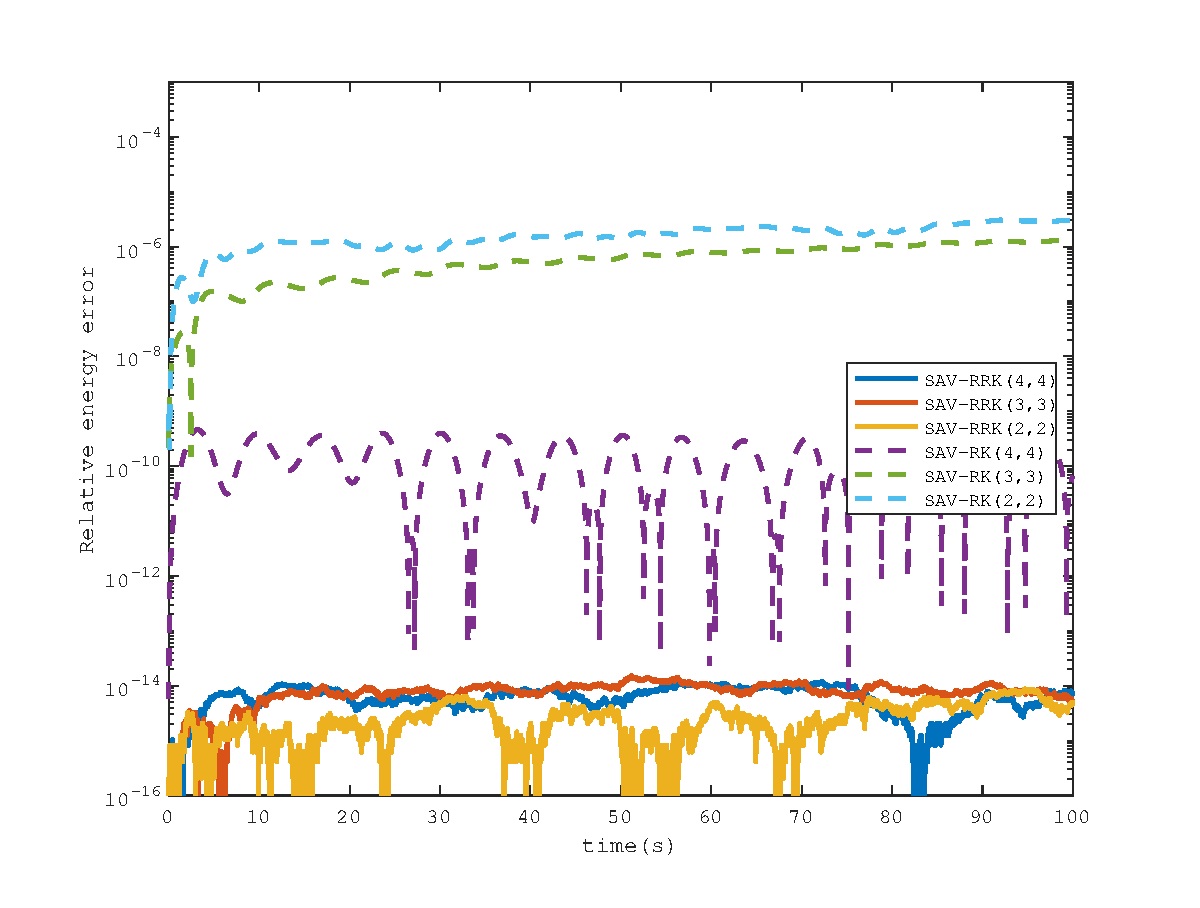
\includegraphics[width=0.5\textwidth]{./figures/exp4_energy6.eps}
%\centerline{($a$) Temporal accuracy with $N=128.$}
}\\
\subfigure[$\alpha,\beta=1.9$]{ \centering
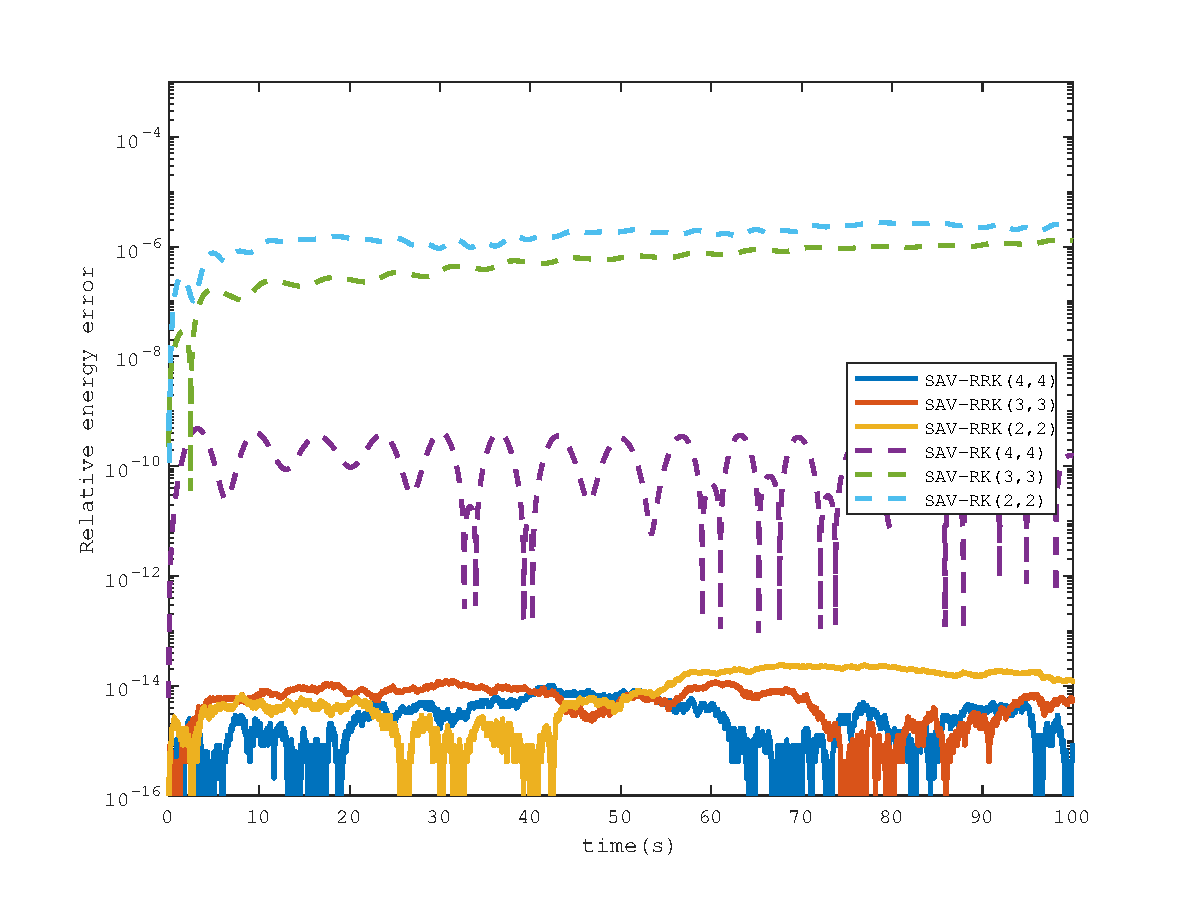
\includegraphics[width=0.5\textwidth]{./figures/exp4_energy9.eps}
%\centerline{($b$) Spatial accuracy with $\tau = 10^{-3}.$}
}\subfigure[$\alpha,\beta=2$]{ \centering
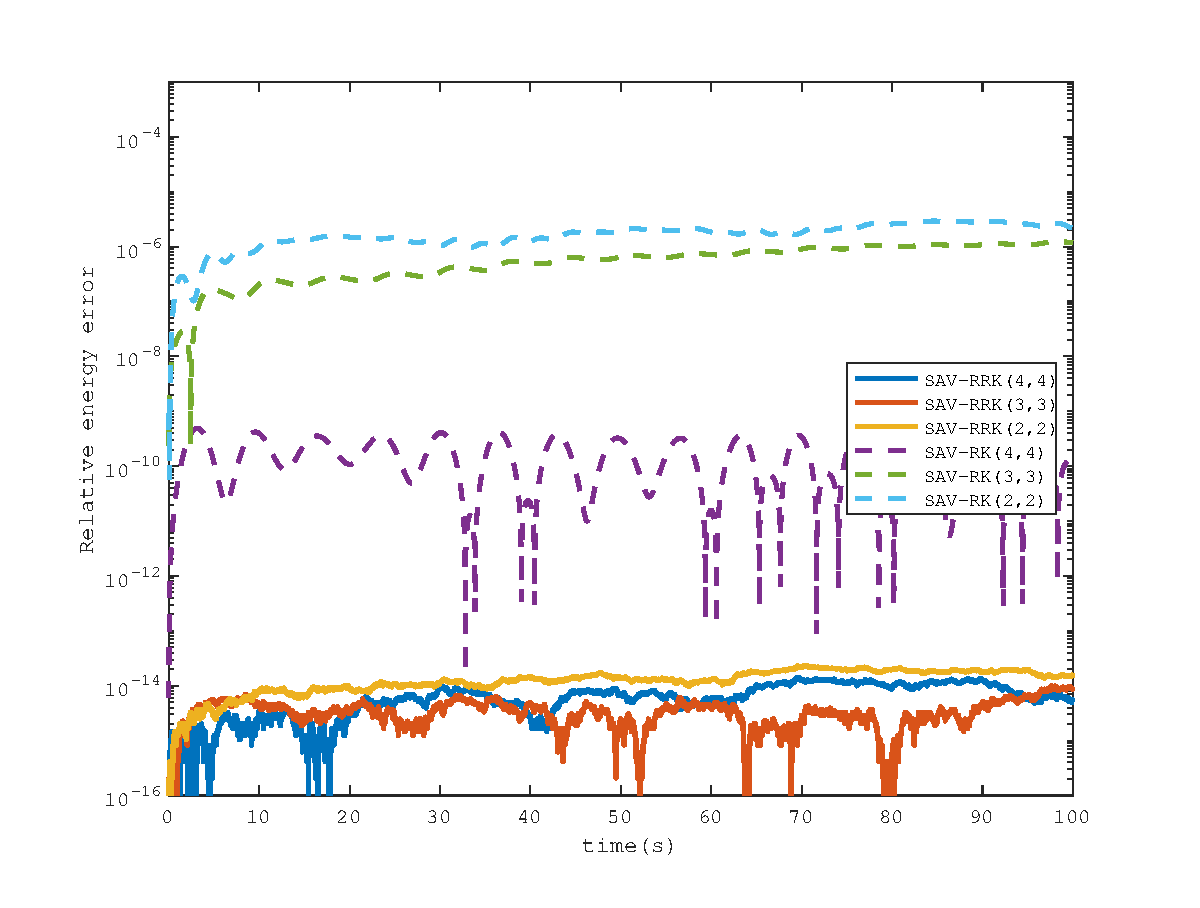
\includegraphics[width=0.5\textwidth]{./figures/exp4_energy2.eps}
%\centerline{($a$) Temporal accuracy with $N=128.$}
}
% \caption{ Relative errors of energy with $N=4, \tau=0.01$ for different $\alpha$ in Example \ref{exp_SAVRRK:4}.}
\caption{当 $N=4, \tau=0.01$ 时,算例 \ref{exp_SAVRRK:4} 取不同 $\alpha$ 对应的相对能量误差.}
\label{fig_SAVRRK:3-5}
\end{center}
\end{figure}

\section{小结}\label{Section_SAVRRK: 7}
本章考虑了具有周期性边界条件的二维非线性分数阶薛定谔波动方程,首先通过标量辅助变量方法将其转化为一个等价系统,其四次形式的能量被重新表述为三个二次项的和.
随后,结合显式松弛龙格库塔方法成功构造了一个在时间方向可达任意高阶的显式能量守恒数值格式.
最后,通过一系列数值实验验证了该格式对于其他类似的守恒问题也是有效的,如分数阶Klein-Gordon-Schr{\"o}dinger方程等,且在长时间仿真中表现出良好的数值稳定性.
